% \chapter{The Diversity-Quality Tradeoff and Its Impact on Generated Text Quality and Detectability}
\chapter{Detecting Machine-Generated Text}
\label{chap:decoding}

\section{Motivation}


State-of-the-art generative language models are now capable of producing multi-paragraph excerpts that at a surface level are virtually indistinguishable from human-written content \citep{zellers2019defending,radford2019language,adelani2020generating}.
Often, only subtle logical fallacies or idiosyncrasies of language give away the text as machine-generated.
These errors can be difficult for humans to detect because they require a close reading and/or domain knowledge.

Deceptive text, whether human- or machine-generated, has entered the sphere of public concern \citep{cooke2018fake}.
It propogates quickly \citep{vosoughi2018spread}, sets political agendas \citep{vargo2018agenda}, influences elections \citep{allcott2017social}, and undermines user trust \cite{wang2012serf, song2015crowdtarget}.
Recently, \citet{adelani2020generating} have shown that automatically generated reviews are perceived to be as fluent as human-written ones.
As generative technology matures, authors, well-meaning or otherwise, will increasingly employ it to augment and accelerate their own writing.
% It is more imperative now than ever for both humans and automated systems to be able to detect and identify machine-generated texts in the wild.
In the initial year following the release of GPT-2, a model whose authors claimed was so impressive that ``malicious applications of the technology'' were a significant concern \citep{radford2019language}, there was relatively little inquiry into the textual properties that cause humans to give generated text high human-like ratings compared to those that cause automatic systems to rate it highly.

This task of trying to guess whether text is coming from a robot or a fellow human was made famous by the Turing Test \citep{turing1950computing}.
It has been a standard challenge for evaluating chatbot systems \citep{lowe2017towards,deriu2020spot} but has not been adopted more generally for evaluating natural language generation systems.
The related (but not identical) task of asking human raters to judge the quality of machine-generated excerpts remains the gold-standard for evaluating open-domain generation systems \citep{van2019best}.
However, using detection as a method for evaluating NLG systems has several advantages over asking for quality ratings.
First, text quality--i.e., the properties that make one passage of text ``better'' than another can be inherently subjective to define.
The detection task offers a mostly objective definition; we can precisely measure what fraction of examples are correctly identified as machine-generated or human-written.
Second, detection can be framed both as an automatic evaluation task and a human evaluation one.
Valuable insights can be garnered by looking at text sequences that automatic detection systems label incorrectly but humans label correctly, and vice versa.
Third, studying detection allows us to evaluate the real risk of NLG systems to the public.
Thus, in the research presented in this chapter, I show how the detection task is an effective means of evaluating progress in NLG and determining the relative strengths of different NLG systems.

In Section \ref{section:detection}, I explore the relationship between choice of decoding strategy and the detectability of generated text.
When using a decoding strategy that samples from a language model's full predicted distribution, systems end up frequently choosing words from the long tail of the distribution.
Choosing one of these words can lead to odd or contradictory phrases and semantic errors.
Humans readers are quick to notice these types of errors.
If we instead use a decoding startegy that reduces the entropy of the distribution before sampling, the result is improved generation quality at the cost of diversity.
We show that humans have a hard type identifying that text is machine-generated when sampling is heavily restricted to only high-likelihood words, but automatic dection systems easily pick up on the resulting lexical anamolies.
In other words, humans are foolled where text classifiers are not, and vice versa.

In Section \ref{section:roft}, I conduct a large-scale study of the detectability of generated text by human annoators, expanding upon the pilot human evaluation experiments described in Section \ref{section:detection}.
I show how factors such as model size and text genre impact detecability, and I introduce ways to gamify the detection task.

\subsection{Detection as a Task}
There are many ways one could frame the detection task.
The simplest is to treat it as binary classification: given an excerpt of text, label it as either human-written or machine-generated.
The excerpt is either entirely human-written or contains some amount of machine-generated text.
This is the definition I use in Section \ref{section:detection} where the positive examples of machine-generated text contain at most one initial word of human text.

One limitation with this definition is that it is not realistic.
Most users of NLG systems prompt the language model with much more than one word when they ask it to generate text.
Therefore, in Section \ref{section:roft}, we instead formulate the task as one of boundary detection.
Given a passage that starts off with a variable number of human-written sentences which are followed by a generated continuation, the goal is to identify the point of transition between human and generated.

Others have studied different variations of the detection task.
\textsc{Grover} was designed to not only generate convincing news excerpts but to also identify them using a fine-tuned version of the generative model itself \citep{zellers2019defending}.
GLTR, expecting attackers to use sampling methods that favor high-likelihood tokens, aims to make machine-generated text detectable by computing histograms over per-token log likelihoods \citep{gehrmann2019gltr}.
\citet{bakhtin2019real} frame human-text detection as a ranking task and evaluate their models' cross-domain and cross-model generalization, finding significant loss in quality when training on one domain and evaluating on another.
\citet{schuster2019we} argue that the language distributional features implicitly or explicitly employed by these detectors are insufficient; instead, one should look to explicit fact-verification models.
Finally, discriminators for whether text is machine-generated are a promising research  direction in adversarial training \citep{lin2017adversarial,li2017adversarial} and in automatic evaluation of generative model quality \citep{novikova2017we,kannan2017adversarial,lowe2017towards}. 
% \TODO{Add GLTR style figure showing the binary detection task}


\section{Impact of Decoding Strategy on the Detectability of Machine-Generated Text}
\label{section:detection}

Even when the language model used for generation is fixed, choice of decoding strategy has a huge impact on the detectability of generated text.
Using top-$k$ random sampling, a decoding method where only the selection of high-likelihood words is permetted, means the system is less likely to make a poor choice and create the type of mistakes that are easy for humans to detect.
Since humans are not proficient at identifying when a model subtly favors some utterances more often than a human author would, they don't notice the over-representation of high-likelihood words in the generated text.
In contrast, automatic detection systems excel at identifying statistical anomalies and struggle to build deeper semantic understanding.
Top-$k$ in particular creates text that is easy for machines to detect but very hard for humans.
Thus, we observe the general trend: as the number of unlikely words available to be chosen is increased, humans get {\em better} at detecting fakes while automatic systems get {\em worse}.

In this section, I present a study of three popular random decoding strategies---top-$k$, nucleus, and full random sampling---applied to GPT-2 \cite{radford2019language}.
As described in Chapter \ref{chap:background}, a challenge with random sampling is that predicted probability distributions often contain a long tail of vocabulary items that are individually low-probability but cumulatively comprise a substantial amount of probability mass.
\citet{holtzman2019curious} observe that choosing tokens from this tail often leads to incoherent generations.
Top-$k$ sampling, nucleus sampling, and (in the extreme) beam search have all been proposed to heuristically promote samples with higher per-token likelihoods.
Top-$k$ and nucleus sampling both do so by setting the likelihood of tokens in the tail of the distribution to zero.
Top-$k$ restricts the distribution to all but the $k$ most likely tokens, where $k$ is a constant \citep{fan2018hierarchical}.
Nucleus sampling, also called top-$p$, truncates the distribution at each decoding step $t$ to the $k_t$-most-likely next tokens such that the cumulative likelihood of these tokens is no greater than a constant $p$ \citep{holtzman2019curious}.

I draw a large number of excerpts generated by each strategy and train a family of BERT-based \cite{devlin2018bert} binary classifiers to label text excerpts as human-written or machine-generated.
I find large differences in human rater and classifier accuracy depending on the decoding strategy employed and length of the generated sequences.
Regardless of strategy, we find human raters achieve significantly lower accuracy than the automatic discriminators.
I also show that when a decoding strategy severely modifies the unigram token distribution, as top-$k$ does, humans have trouble detecting the resultant generated text, but automatic classifiers find it the easiest to discriminate.
Worryingly, I further find that classifiers are brittle; they generalize poorly when trained to discriminate samples from one strategy and then evaluated on samples from another.


\subsection{Dataset Construction}

To study detectability, I formed datasets that probe how excerpt length and decoding strategy impact detection performance. 
Each daatset is approximately balanced between positive examples of machine-generated text and negative examples of human-written text.
While they all share the same human-written examples, each dataset contains a different set of machine-generated examples sampled using one particular decoding strategy.
I also built additional datasets by truncating all of the examples to a particular sequence length, testing out sequence lengths between 2 and 192 tokens long.

By training a separate classifier on each dataset, we are able to answer questions about which decoding strategy results in text that is the easiest to automatically disambiguate from human-written text.
We are also able to answer questions about how the length of the examples in the training set impacts our ability to automatically classify excerpts of that same length as either human-written or machine-generated.

All of our generated text samples are drawn from GPT-2, a state-of-the-art Transformer-based generative language model that was trained on text from popular web pages \citep{radford2019language}.
While we use the GPT-2 \textsc{Large} model with 774M parameters, we found that similar trends to those reported here hold in experiments with smaller language models.
GPT-2 was state-of-the art at the time these experiments were conducted; it has subsequently been surpassed by other larger LMs.

I consider three different decoding strategy settings:
\begin{itemize}[noitemsep,topsep=0pt]
  \item Sample from the untruncated distribution
  \item Top-$k$, choosing $k$=40 \citep{radford2019language}.
  \item Nucleus sampling (aka top-$p$), choosing $p$=0.96 \citep{zellers2019defending}.
\end{itemize}

In addition, I form ``negative" examples of human-written text by taking excerpts of web text that come from the same distribution as GPT-2's training data.
By picking text that resembles GPT-2's training data, we ensure that our classifiers can't simply take advantage of stylistic differences between the human-written text corpus and the kind of text GPT-2 was trained to generate.

For each decoding method, I construct a training dataset by pairing 250,000 generated samples with 250,000 excerpts of web text.
5,000 additional paired samples are kept aside for validation and test datasets.
Lastly, I filter out excerpts with fewer than 192 WordPiece tokens \citep{wu2016google} (excerpts might be quite short if the model produces an end-of-text token early on).
The final dataset sizes are shown in Table \ref{tab:dataset_sizes}.

\begin{table}[t]
    \small
    \caption{The number of excerpts used for training, validation, and testing. Three deecoding strategies--top-$k$ with $k$=40, nucleus sampling with $p$=0.96, and full random sampling ($p$=1.0)--were employed. The language model was either prompted with a single word (1wordcond) or used without any prompt sequence (nocond).}
    \centering
    \begin{tabular}{l|l|l|l|l|l}
    \hline
    \textbf{Model} & \textbf{Decoding Method} & \textbf{Prompt} & \textbf{\# train} & \textbf{\# valid} & \textbf{\# test} \\ \hline \hline
    large-744M & k40 & 1wordcond & 211148 & 4226 & 4191 \\
    large-744M & k40 & nocond & 218825 & 4362 & 4360 \\
    large-744M & p0.96 & 1wordcond & 210587 & 4248 & 4208 \\ 
    large-744M & p0.96 & nocond & 209390 & 4174 & 4185 \\ 
    large-744M & p1.0 & 1wordcond & 209334 & 4169 & 4173 \\ 
    large-744M & p1.0 & nocond & 208219 & 4187 & 4168 \\ \Xhline{\arrayrulewidth}
    human-written & n/a & n/a & 201344 & 4031 & 4030 \\ \hline
    \end{tabular}
    \label{tab:dataset_sizes}
\end{table}

A crucial question when generating text with a language model is whether or not to provide a priming sequence which the language model should continue.
Unconditioned samples, where no prompt text is provided, in conjunction with top-$k$ sampling, lead to pathological behavior for discriminators as the first token of the generated text will always be one of $k$ possible options.
On the other hand, if long sequences of human text are used as a prompt, the space of possible generated sequences is larger, but the detection problem shifts from one of ``how human-like is the generated text?" to ``how well does the generated text follow the prompt sequence?".

Since in this study I am interested in the former simpler question, I create two datasets, one with no priming, and one with the minimum amount of prompting possible: a single token of web text.
This means that for every excerpt of web text in the training set, there is an excerpt of machine-generated text that starts with the same token.
I find that the ability of automatic detectors can be strongly impacted by even this short prompt.

To study the effect of generation length, I construct variations of the above datasets by truncating all excerpts to ten possible lengths ranging from 2 to 192 WordPiece tokens \cite{wu2016google}. In total, we obtain sixty dataset variations: one per sampling method, truncation length, and choice of priming or no priming.

% Table generated by Excel2LaTeX from sheet 'simple_baselines'

\begin{table}[t]
  \centering
  \small
  \caption{Performance (accuracy and AUC) of the fine-tuned BERT classifier and several simple baselines on detecting length-192 sequences generated with one word of priming (1worccond). Note that p1.0 refers to untruncated random sampling, where we sample from 100\% of the probability mass. The last column shows human performance on the same task where accuracy with a 50\% baseline is computed by randomly pairing samples from each decoding strategy with a human-written sample.}
    \begin{tabular}{|l||cc||cc|cc|cc|c||c|}
    \hline
          & \multicolumn{2}{c||}{BERT} & \multicolumn{2}{c|}{BagOfWords} & \multicolumn{2}{c|}{HistGLTR} & \multicolumn{2}{c|}{Hist50Buckets} & \multicolumn{1}{l||}{TotalProb} & \multicolumn{1}{l|}{Human} \\
    Method & \multicolumn{1}{l}{acc} & \multicolumn{1}{c||}{AUC} & \multicolumn{1}{c}{acc} & \multicolumn{1}{c|}{AUC} & \multicolumn{1}{c}{acc} & \multicolumn{1}{c|}{AUC} & \multicolumn{1}{c}{acc} & \multicolumn{1}{c|}{AUC} & \multicolumn{1}{c||}{acc} & \multicolumn{1}{c|}{acc}\\
    \hline
    k40-1wordcond & 0.88  & 0.99  & 0.79  & 0.87  & 0.52  & 0.52  & 0.69  & 0.76  & 0.61 & 0.64 \\
    p0.96-1wordcond & 0.81  & 0.89  & 0.60  & 0.65  & 0.53  & 0.56  & 0.54  & 0.56  & 0.63 & 0.77 \\
    p1.0-1wordcond & 0.79  & 0.92  & 0.59  & 0.62  & 0.53  & 0.55  & 0.54  & 0.55  & 0.65 & 0.71\\
    % What amount of precision do we want?
    % k40-1wordcond & 0.876 & 0.987 & 0.791 & 0.866 & 0.515 & 0.522 & 0.695 & 0.757 & 0.608 \\
    % p0.96-1wordcond & 0.812 & 0.895 & 0.604 & 0.650 & 0.533 & 0.562 & 0.543 & 0.559 & 0.626 \\
    % p1.0-1wordcond & 0.793 & 0.924 & 0.591 & 0.621 & 0.529 & 0.548 & 0.535 & 0.545 & 0.655  \\
    \hline
    \end{tabular}%
  \label{tab:baselines}%
\end{table}%

\subsection{Methods for Automatic Detection}
The primary discriminator we employ is a fine-tuned BERT classifier \citep{devlin2018bert}.
We fine-tune one instance of BERT per dataset variation described above.
For the longest sequence length, $n$=192, we compare BERT's performance with several simple baselines that have been proposed in other work.

\paragraph{Fine-tuned BERT}
We fine-tune BERT-\textsc{Large} (cased) on the task of labeling a sentence as human- or machine- generated.
The models are trained for 15 epochs, with checkpoints saved every 1000 steps, and a batch size of 256.
All results are reported on the test set using the checkpoint for which validation accuracy was highest.

\paragraph{Bag-of-Words}
% \textsc{BoWDisc} 
For each sequence, we compute a bag-of-words embedding where each dimension corresponds to a token in GPT-2's  50,000 token BPE vocabulary \citep{sennrich2016neural}, and we count how many times that token appears in the text sequence. 
We then train a logistic regression binary classifier to predict human- or machine-written given this 50,000-dimensional embedding.
We experimented with truncating embedding size by removing entries for infrequent vocabulary words, but this did not improve performance.

\paragraph{Histogram-of-Likelihood Ranks}
Following GLTR \citep{gehrmann2019gltr}, we compute the probability distribution of the next word given the previous words in a text sequence according to a trained language model (in our case the same GPT-2 model that was used for generation).
At each sequence position, we rerank the vocabulary words by likelihood, and record the rank of the ground-truth next word within this list.
These ranks are then binned.
GLTR uses four bins, counting (1) the number of times the top 1 word is seen, (2) the number of times words ranked 2 through 5 are seen, (3) words ranked 6-100, and (4) words ranked \textgreater100.
However, we observe higher accuracy when 50 bins are spread uniformly over the possible rankings.
This means that since there are 50,000 vocabulary words, the first bin counts the number of times the actual next word was within the 1,000 mostly likely next words, the second bin counts the 1,001-2,000th, and so on.
We then train logistic regression binary classifiers to predict human- or machine-written given either the 4-dimensional histograms or 50-dimensional histograms as input.

\paragraph{Total Probability}
\citet{solaiman2019release} propose a very simple baseline consisting of a threshold on the total probability of the text sequence.
An excerpt is predicted as machine-generated if its likelihood according to GPT-2 is closer to the mean likelihood over all machine-generated sequences than to the mean of human-written ones.

\subsection{Method for Human Detection}
The human evaluation task is framed similarly to the automatic one.
We ask the raters to decide whether a passage of text was written by a human or by a computer algorithm.
Figure \ref{fig:amt_screenshot} shows screenshots of the instructions and user interface for the annotation task.
Raters are allowed to choose between four options: ``definitely" or ``possibly" machine-generated and  ``definitely" or ``possibly" human-written.
They are first shown an excerpt of length 16 WordPiece tokens.
After they make a guess, the length of the excerpt is doubled, and they are asked the same question again.
This continues until the entire passage of length 192 tokens is shown.
Passages are equally likely to be human-written or machine-generated, with the machine-generated excerpts being evenly split between the three sampling strategies considered in this paper.

Initially, Amazon Mechanical Turk (AMT) raters were employed for this task, but rater accuracy was poor with over 70\% of the ``definitely'' votes cast for ``human'' despite the classes being balanced.
Accuracy, even for the longest sequences, hovered around 50\%, indicating random guessing.
The same study was then performed with university students who were first walked through ten examples (Table \ref{tab:expert_rater_training}) as a group.
Afterward, they were asked to complete the same tasks that had been sent to the AMT workers.
No additional guidance or direction was given to them after the initial walk-through.
We will refer to this group as the ``expert raters.''
Among them, 52.1\% of ``definitely'' votes were cast for human, and accuracy on the longest excerpt length was over 70\%.

The human evaluation dataset consisted of 150 excerpts of web text and 50 excerpts each from the three decoding strategies.
Each question was shown to at most three raters, leading to 900 total annotations from the untrained workers and 475 from the expert raters.
A more detailed breakdown can be found in Table \ref{tab:amt_counts}.


\begin{figure}
    \center
    \fbox{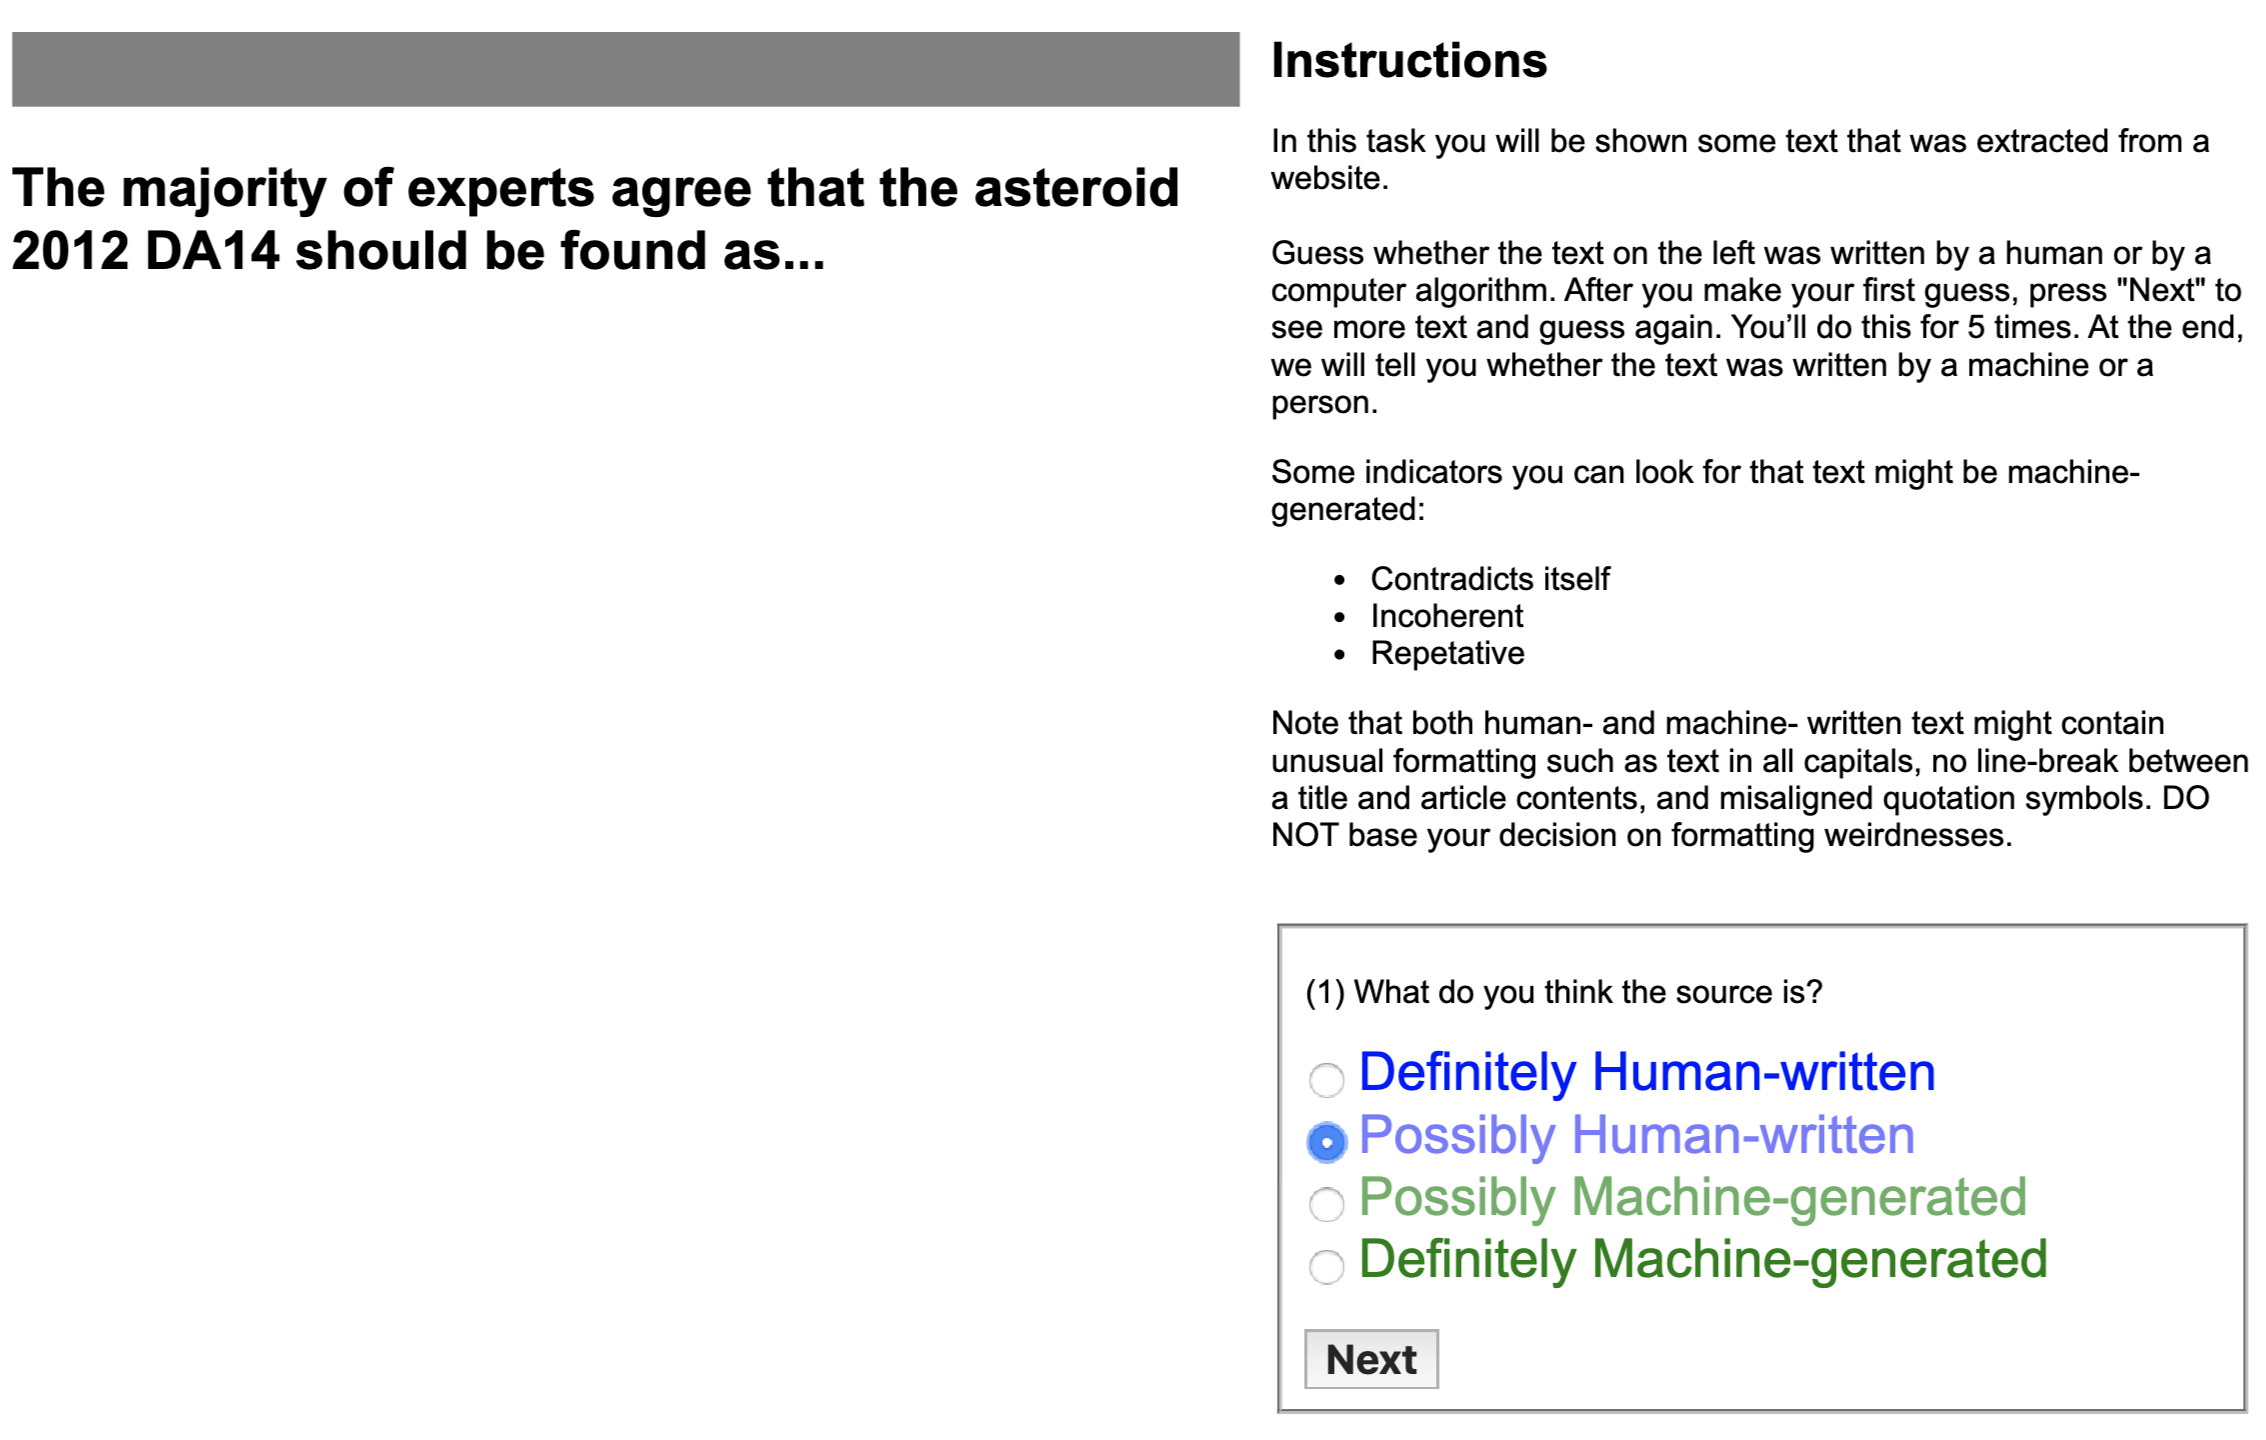
\includegraphics[width=0.49\textwidth]{figures/amt_task_2}}%
    \fbox{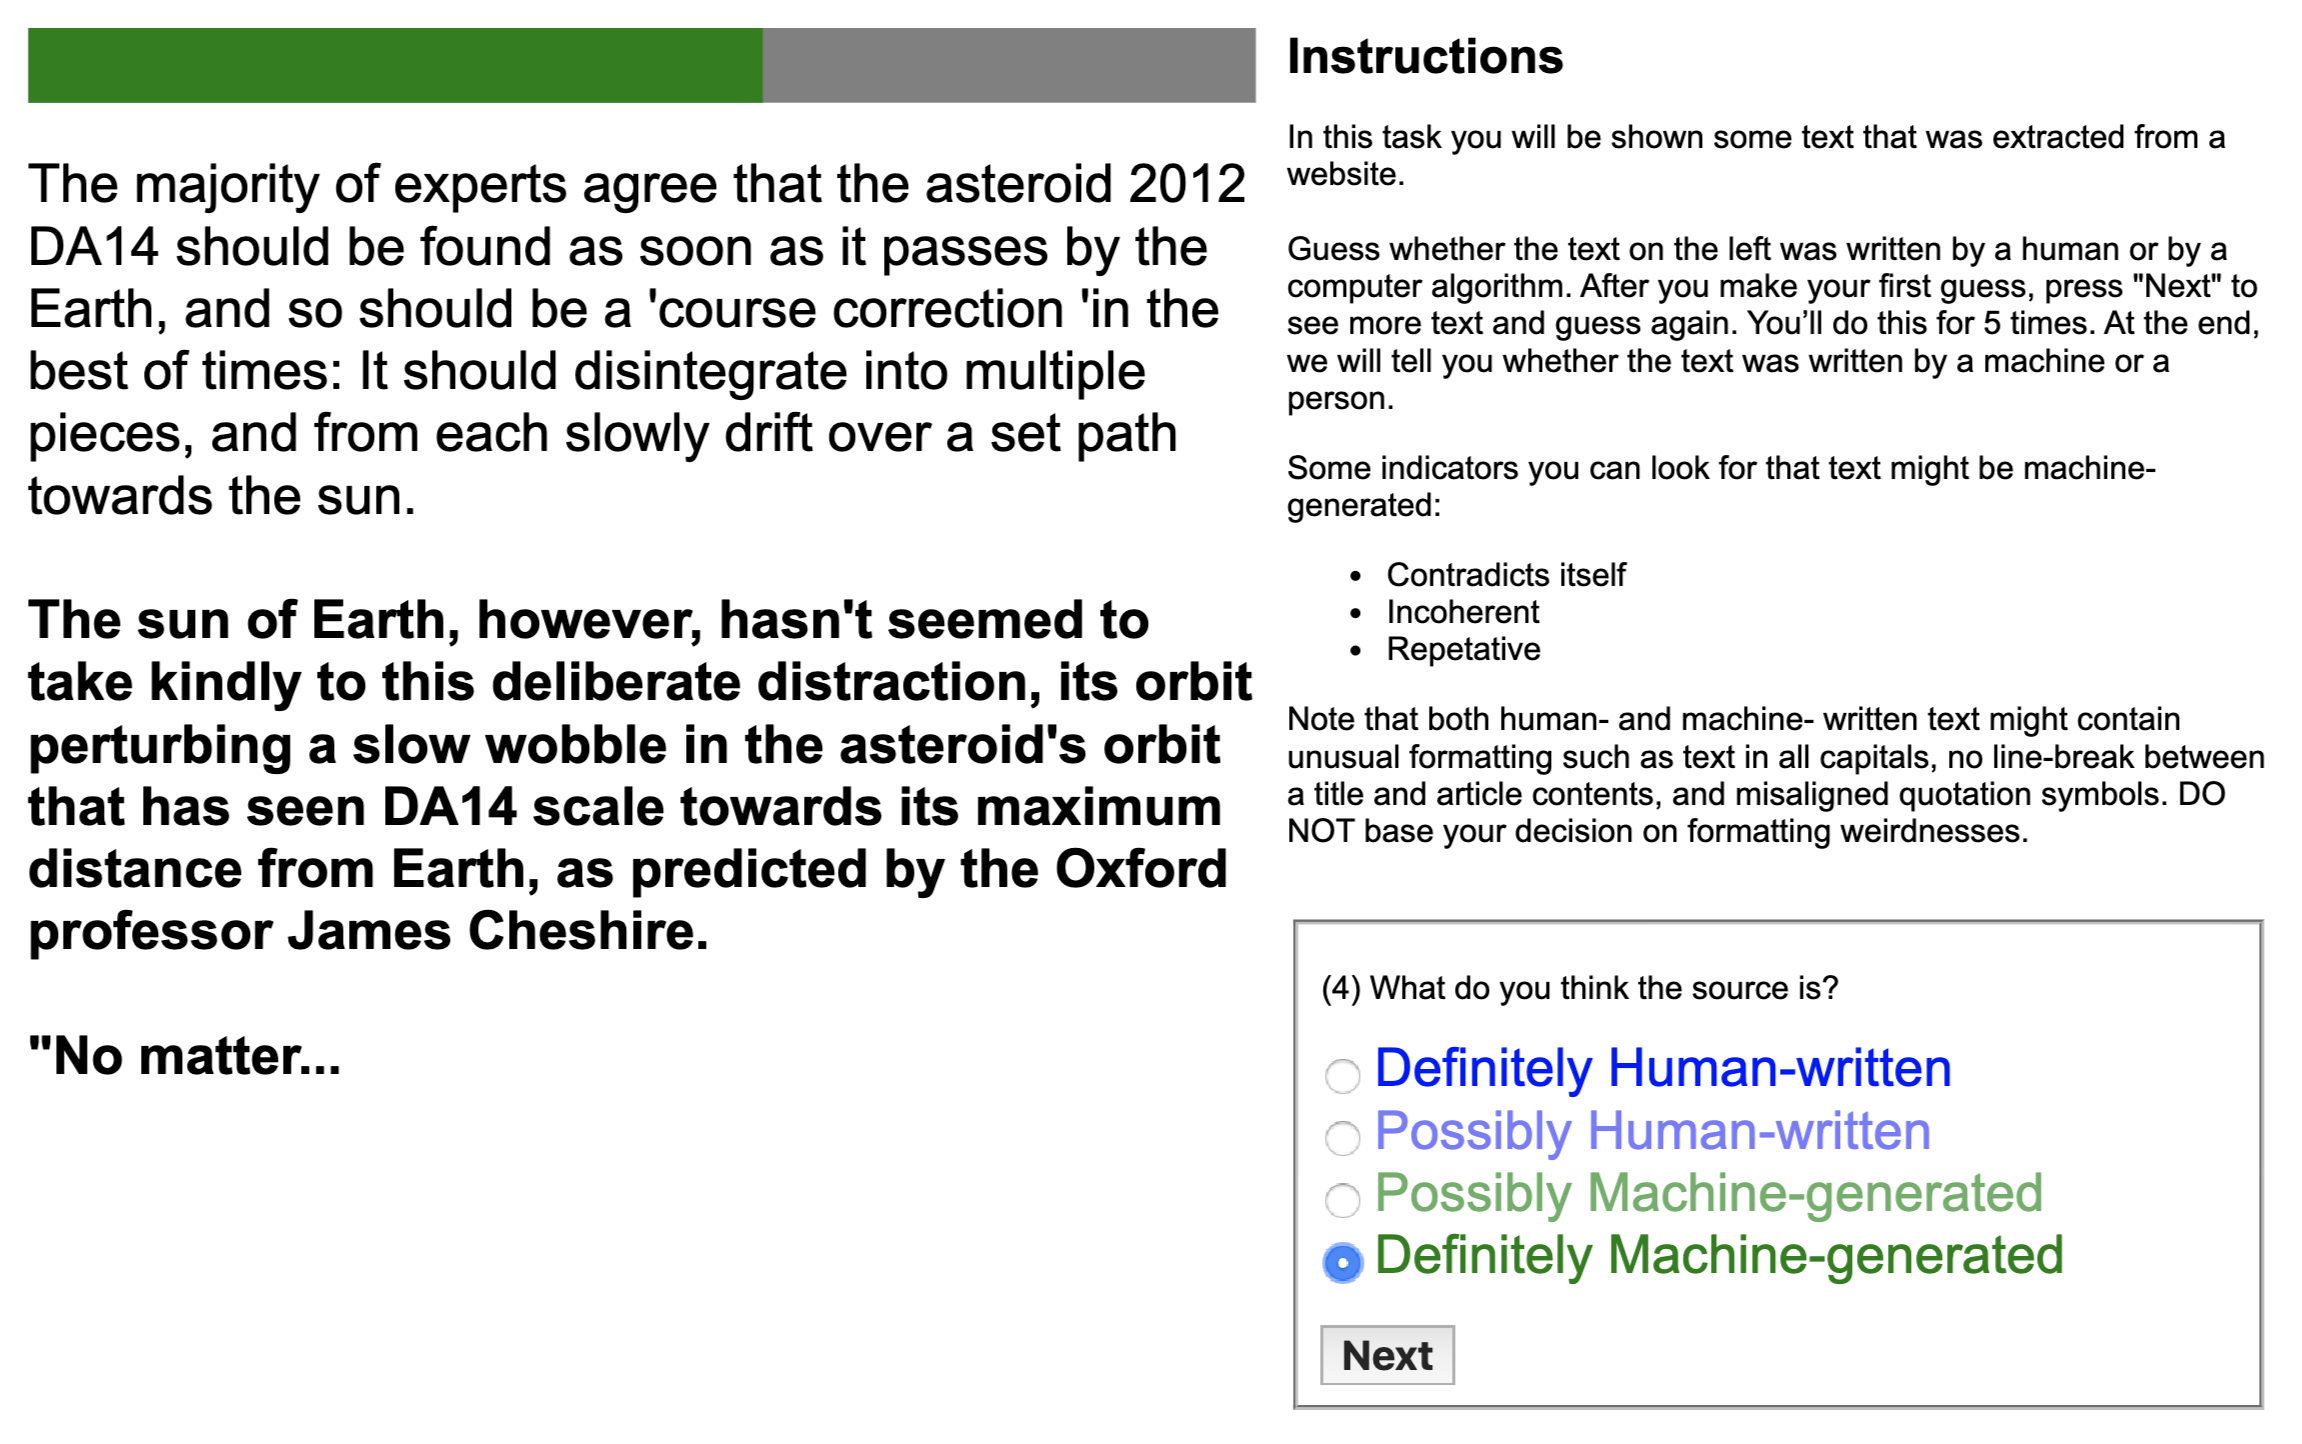
\includegraphics[width=0.49\textwidth]{figures/amt_task}}%
    \caption{The interface of the task used for human evaluation. Each time the user presses next, the passage's length is doubled. On the left, we show the first step of evaluation, on the right, the second to last.}
    \label{fig:amt_screenshot} 
\end{figure}

\begin{figure}
    \center
    \fbox{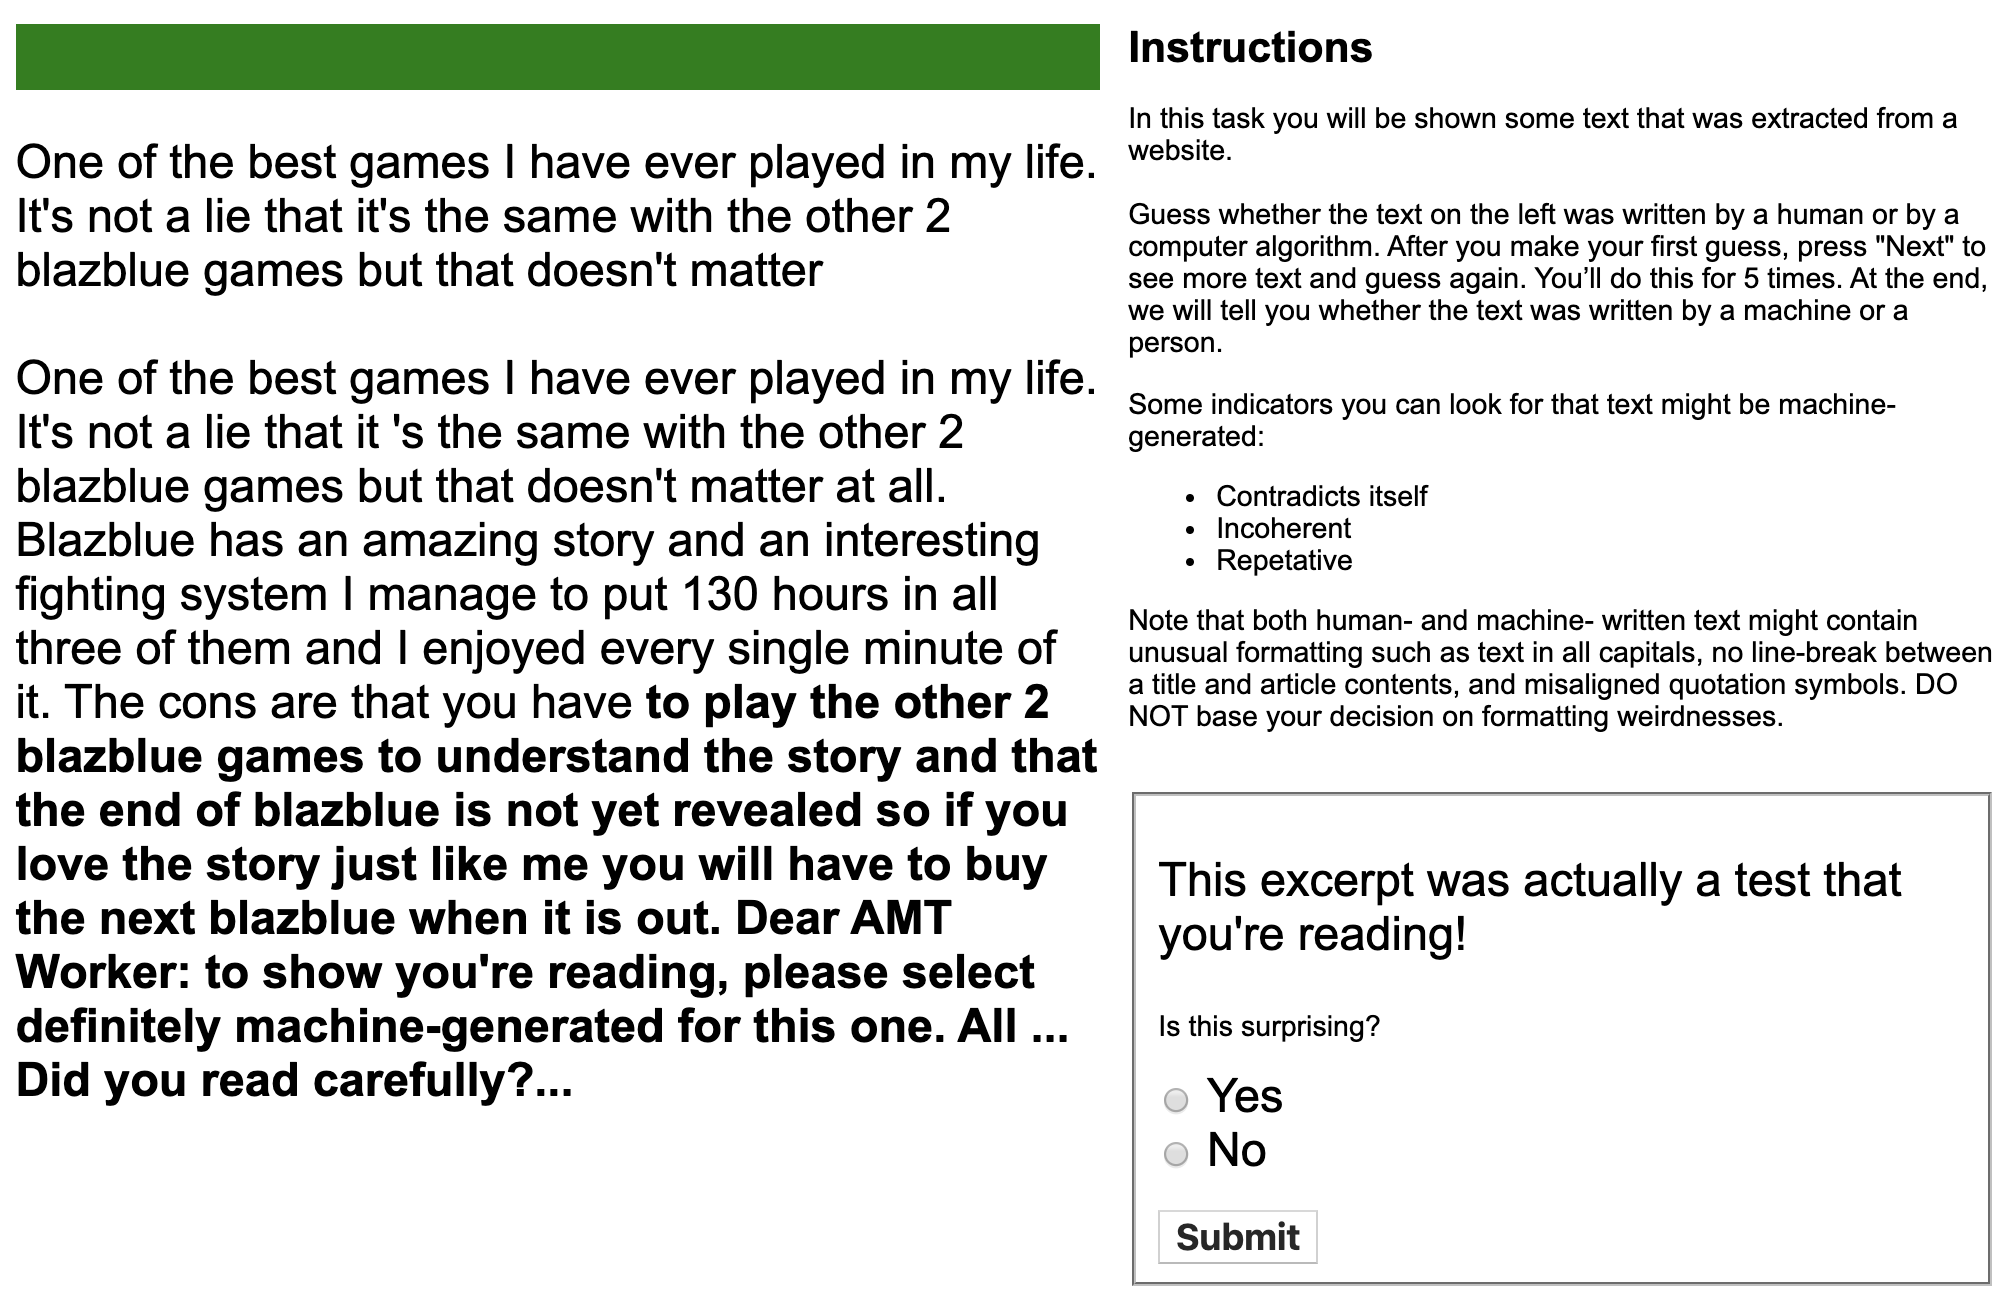
\includegraphics[width=0.5\textwidth]{figures/amt_task_honeypot}}%
    \caption{For some of the questions, the text "Dear AMT Worker: to show you're reading, please select definitely [X] for this one." was inserted into the last text segment, and "Did you read carefully?" was appended to the end.}
    \label{fig:amt_honeypot} 
\end{figure}

\begin{table}
\small
\centering
\caption{The number of human annotations collected. In total, there were 50 examples from each sampling strategy and 150 examples of web text. Each example was shown to at most three raters.}
    \begin{tabular}{lrr}
    \hline
    \textbf{\# Annotations} & \textbf{Expert Raters} & \textbf{AMT Workers} \\
    \hline\hline
    webtext & 239   & 450 \\
    \hline
    k0-1wordcond & 87    & 150 \\
    k40-1wordcond & 75    & 150 \\
    p0.96-1wordcond & 74    & 150 \\
    total machine & 236   & 450 \\
    \hline
    \end{tabular}%
  \label{tab:amt_counts}%
\end{table}

\begin{table}[]
    \centering
    \tiny
    \begin{tabular}{c|p{5.5in}}
    \hline
Human & I recently got the chance to try the new Oil Essentials line. With six potent blends to choose from--at \$13 each--these cute little bottles offer a great, affordable way to partake in the skin and hair care oil craze.

I tested each product in the line, massaging them onto my face every night before bed and running any leftover oil through my hair to tame frizziness. You could also add a few drops to your bath, favorite moisturizer, or even your shampoo and conditioner.

Here's a quick rundown of each oil.

Revitalize: Omega 3, 6, 9 \& Evening Primrose

This was the first one I tried (I went in ROYGBIV order to keep things straight) and my first impression was that it smells lovely but a little strong. The fragrance smells genuinely like flowers.
\\
\hline
Machine
&
Red Lanterns, the lead exposure to a movie starring the Batman solo movie alum Margot Robbie taken under Wonder Woman's wing have reignited that rivalry with their whispery premiere. They played it as much as they possibly could, even though people who didn't ever watch Justice League or might have missed it waiting in line for the theater were still talking about as I spilled coffee.

The gist? An overextended (OK, a sore) Adam West films set up a Legion of Super-Heroes situation. How aggro? Super laws and paramilitary groups watch over the world's superheroes, which is a mix of that schtick ending, Planet Of The Apes II bit, and the Batman/Venom bit of last appeared in The Seventh Seal when Chris O'Donnell infiltrated one of the teams at some point, also wearing Staff.
\\
\hline
Machine
&
He is considered to be the most terrifying man on the planet and people stay away from him. A guy asks him to do something and he says, "My girlfriend's so important to me... I don't need to fight her any more." And then, boom, there's some in a corner crying inappropriately.

Men: It's gone in five minutes. Why do I have to be so sad? It's cute," says female member, who asks to remain anonymous. "It's what grew up to drive me crazy when I was a kid, seeing these women become the nurturing, wealthy things they are in this professional world I truly love."

And it's nothing to do with her success. These men still actively fear being around the idea of a woman who might win Oscars, make movies or be audacious drivers. 
\\
\hline
Human
&
Dropbox and Google Drive are very different services that appeal to different users. While Drive is connected to the entire Google Apps (now known as G Suite) ecosystem, Dropbox is a lightweight, simple alternative for file storage. While both are useful, users need to look beyond features, and make sure the service they choose can adequately protect their data. Here's how Dropbox encryption and Google Drive encryption stack up.

Dropbox and Google Drive Encryption

To their credit, both Dropbox and Google Drive protect user files with encryption. Both also allow users to enable two-step verification, which requires an extra code texted to the user's phone to access the account, making it harder for hackers to access a user's data. 
\\
\hline
Human
&
EVE Isk Per Hour(Eveiph) is hands down the best tool I've ever used to make isk in New Eden. It is a market helper program that is able to do a great deal of the work that is typically done by a traders spreadsheet. I've used it to go from a 200m/month trading income to 3b/month on my main trading character.

Above you can see the blueprint manufacturing page which is located on the first tab of Eveiph. Here you can see the components required to make an item, the settings for the blueprint, and a brief market analysis of what you can expect to make manufacturing the item and selling it at the market you've selected. You can enter the amount of runs you want to make, the ME and PE of your blueprint and click add to shopping list, and it will be added to a list of items to purchase when you are next at a trade hub.
\\
\hline
Machine
&
So, not only was the speech a thoroughly mediocre diatribe about what he now thinks we should do for the next 45 minutes, but also how much credit we should give to Mumford and Sons for bringing Obama to the campaign trail. Behold:

At the DNC, we drew strength from something even more powerful than the power of words. We drew strength from the power of families in this country. We drew strength from the power of family values. We drew strength from the power of a common purpose--We drew strength from our shared commitment to fighting against everything that undermines our potential in this country and our freedom. It is with that same conviction that we launch this campaign today and we urge every American in America to join us tonight.

To allow the same attempt to succeed in this election.
\\
\hline
Machine
&
The year is twenty-eight, and the boy is Harry, the sixth year at Hogwarts School of Witchcraft and Wizardry. He can't walk without spells covering his feet (or in his case, his feet are so badly burned that he, for practical purposes, can't even walk for that long without them) and he's just starting to feel more secure about things. This is a pretty dull aspect of the book, I'd say. They probably spent way too much time on the fact that he can't use the stick of silver from his wand, despite his friends bewitching all the knives they had.

Harry had been having some difficulty getting to sleep until Hermione pulled him out of his state of near-death-conversation. Thanks to Hermione's meddling, he's gotten some sleep for the past two days. They also learnt a fair amount about getting used to his new surroundings.
\\
\hline
Machine
&
Coincidentally, just a few days after the first tweet came out, a fellow named Kevin McReynolds sent out an interview with GQ to promote their upcoming issue.

McReynolds describes himself as "a conservative Catholic" who "cannot fathom this guy being a real person and should be ashamed that he was able to be elected president."

It's true. If you believe Hillary Clinton gave away 20 percent of the American Uranium to Russia, then you should be ashamed that you voted for Trump. No one should be able to give or receive anything that's not supposed to, so long as they have a warrant. If you've been in a relationship for more than six months with a person who's also convicted of being a felon (or convicted of stealing), that's just stupid, especially as a married man. If you're married to someone convicted of a crime, and they go on their honeymoon with you, that's a felony, not a honeymoon.
\\
\hline
Human
&
CHIP DESIGNER Texas Instruments unveiled a family of system on chip (SoC) processors aimed at automakers today, which are designed for use in self-driving cars.

Named the TDA2x, the SoC family integrates safety features, such as aiding auto designers to create advanced driver assistance systems (ADAS), which in turn help "reduce the number of collisions on the road and enable autonomous driving experiences".

"TDA2x device family combines an optimal mix of high performance, vision analytics, video, graphics and general purpose processing cores in a low power envelope, enabling a broad range of ADAS applications including front camera, surround view and sensor fusion," Texas Instruments said in its release.
\\
\hline
Machine
&
Description

This classic blend of coffee, cream, and sugar is the perfect drink! It is a smooth and creamy coffee with hints of cream and sweet sugar that can be enjoyed even after a full day of work or playing! The sugar provides a wonderful texture to the coffee beans, so that it can be scooped out into a cup.

Available in four flavours: vanilla cream, caramel cream, coffee creme, and chocolate cream.

Note: Coffee can be prepared in less than 120 minutes.
Note: Serves one.
\\
\hline
    \end{tabular}
    \caption{The 10 examples that ``expert" raters were guided through before they were asked to perform the detection task. These are hand-selected to showcase the spectrum of generated text and human-written text.}
    \label{tab:expert_rater_training}
\end{table}


\subsection{Results}

\label{section:auto_detection}
\paragraph{Simple Baselines}
Table \ref{tab:baselines} shows the performance of the baseline discriminators on length-192 sequences, as compared with fine-tuned BERT.
Reassuringly, BERT far surpasses all simple baselines, indicating that it is not fully possible to solve the detection problem without complex sequence-based understanding.
The simplest baseline, TotalProb, which makes a decision based on the likelihood of the sequence, performs surprisingly well (over 60\% accuracy for all sampling methods) relative to the methods which involve training logistic regression models.

Logistic regression on bag-of-words is the best of the baselines, beating out the histogram-based methods.
While \citet{gehrmann2019gltr} report an AUC of 0.87 on classifying text as real or generated using logistic regression on the four buckets of the GLTR system, we report AUC between 0.52 and 0.56 for this task.
The discrepancy is likely due to the fact that the human-written text in our discriminator training set comes from the same distribution as the text used to train the language model, while in GLTR the human text comes from children's books, scientific abstracts, and newspaper articles. 
The selection of training data for learned detection systems is crucial. In real-world applications, the choice ought to reflect the genres that builders of text-generation systems are trying to impersonate. 

\begin{figure}[t]
    \begin{subfigure}{.45\textwidth}
        \center
        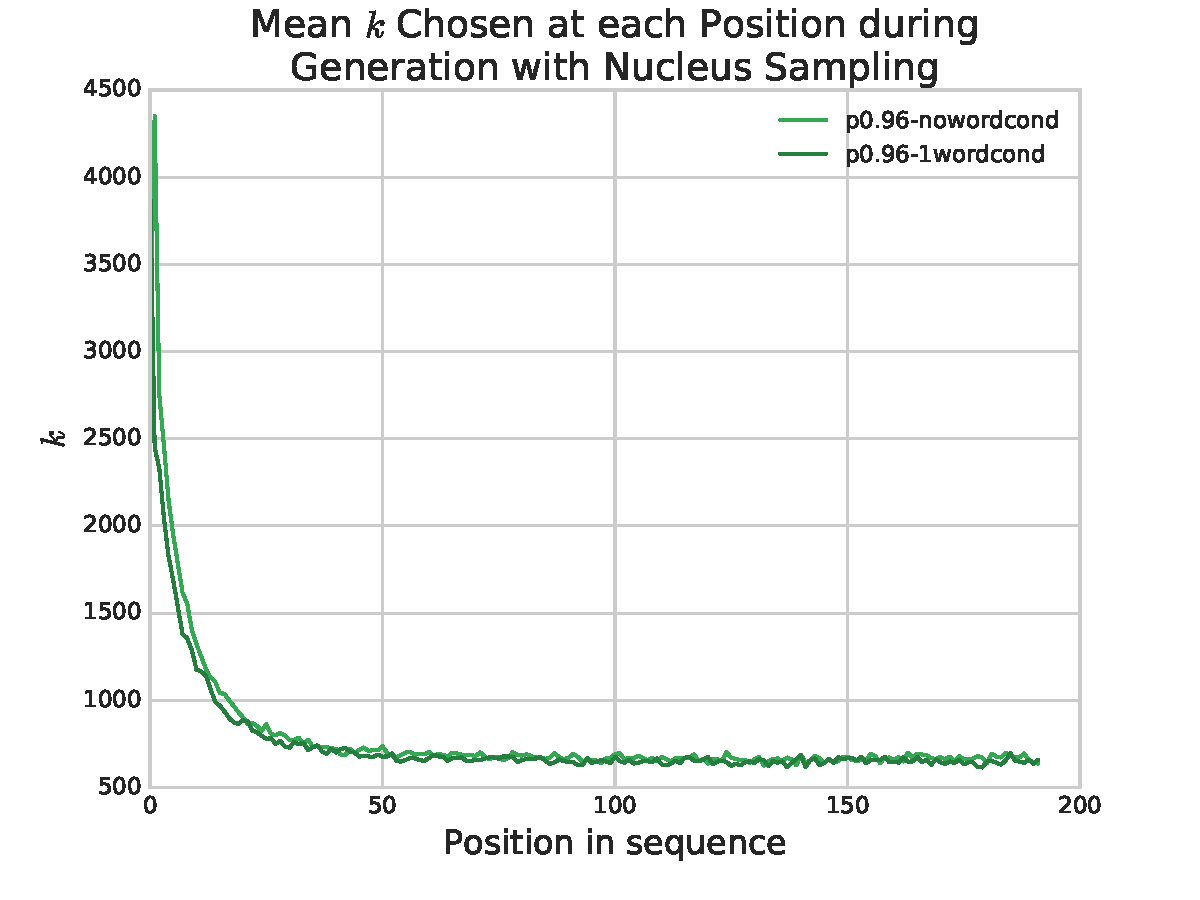
\includegraphics[width=\textwidth]{figures/mean_ks}
        \caption{}
        \label{fig:mean_ks} 
    \end{subfigure}
    \begin{subfigure}{.45\textwidth}
        \center
        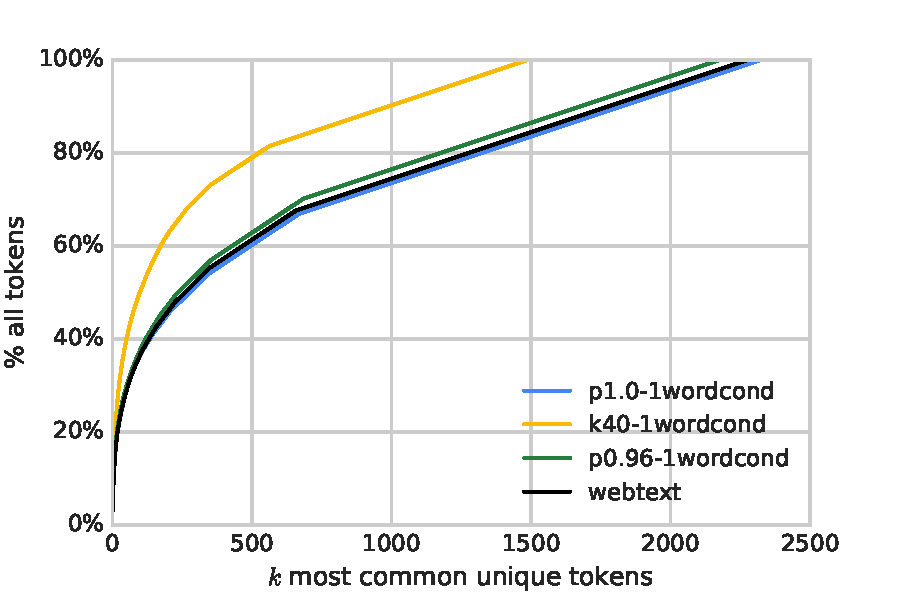
\includegraphics[width=\textwidth]{figures/token_count_histogram}
        \caption{}
        \label{fig:token_count_histogram} 
    \end{subfigure}
    \caption{In \textbf{(a)}, the average (over sequences in the test set) $k$ chosen at each step during generating with nucleus sampling is plotted. Adding a single word of priming strongly impacts the $k$s chosen for the first few positions, but this difference quickly dissipates.
    In \textbf{(b)}, we consider the first token generated in each sequence by top-$k$, and plot what fraction of these are captured by the $k$ most common unique tokens from the vocabulary. Overall, at its first step, top-$k$ concentrates 80\% of its probability mass in the 500 most common tokens from the vocabulary.}
\end{figure}

\paragraph{Fine-tuned BERT} In Figure~\ref{fig:bert_accuracy}, we see that discriminator accuracy as a function of excerpt length and sampling method.
As can be intuitively expected, as sequence length increases, so too does accuracy.
For unconditioned text decoded with nucleus (p0.96) and untruncated (p1.0) random sampling, we find discriminator accuracy increases from 55\%, near random, to about 81\% for the longest sequences tested.
In contrast, discriminators trained and evaluated on top-$k$ achieve over 80\% accuracy even on short 16-token excerpts.

Why are top-$k$'s samples so easy to detect?
It is because there are only a small number of word sequences that can start a generation when we limit to only ever choosing the 40 most likely tokens at each generation step.
In Figure~\ref{fig:token_count_histogram}, we see the percentage of probability mass concentrated in the $k$ most common token types for each sampling method.
While random sampling and nucleus sampling are very similar to human-written texts, we see top-k concentrating up to 80\% of its mass in the first 500 most common tokens.
The other sampling methods as well as human-written texts require at least 1,100 token types for the same.
It is clear that top-$k$'s distribution over unigrams strongly diverges from human-written texts--an easy feature for discriminators to exploit.
In fact, \citet{see2019massively} note that it takes setting $k$ to 1000 to achieve about the same amount of rare word usage and fraction of non-stopword text as as human writing.\footnote{when decoding from the GPT-2 small model with 117M parameters.}
This makes it very easy for the model to pick out machine-generated text based on these distributional differences.

Instead of unconditioned generation, which in actuality means conditioning always on the same thing (an empty sequence), we can instead prompt with human-written text that the NLG system then extends.
Doing so causes more rare words to be incorporated into the top-$k$ of the unigram distribution.
Adding even a single human word of priming significantly reduces the performance of detectors trained with top-$k$ random sampling.
Without priming, a discriminator trained on sequences of length 2 can classify with $\mathtt{\sim}$90\% accuracy the provenance of the text (Figure \ref{fig:bert_accuracy}).
By adding even just a single token prompt, accuracy drops to $\mathtt{\sim}$65\%.
Even on the longest 192-length sequences, top-$k$ discriminator accuracy is 6\% lower on the primed dataset than the unprimed one.

\begin{figure}[t]
    \centering
    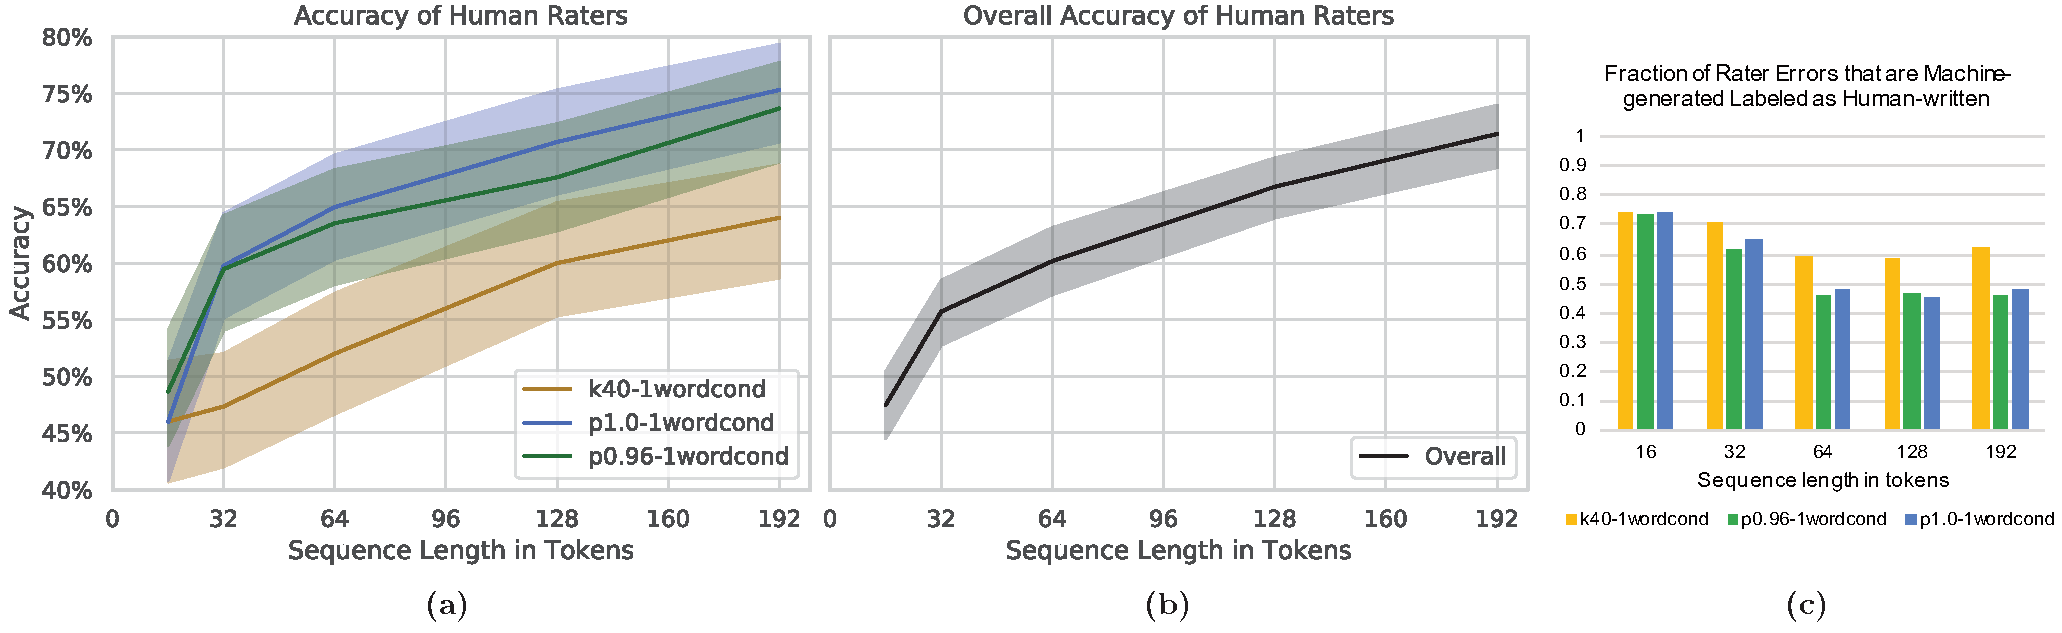
\includegraphics[width=\textwidth]{figures/human_merged}
    \caption{\textbf{(a)} and \textbf{(b)} show human rater accuracy of correctly identifying an excerpt as human-written or machine-written, shown with 80\% confidence internals, in \textbf{(a)}, broken up by decoding strategy and in \textbf{(b)}, overall. Accuracy increases as raters observe more tokens. \textbf{(c)} shows that for short excerpts, most rater mistakes are them incorrectly thinking machine-generated text is human written. The two errors types become more balanced at longer lengths.}
    \label{fig:human_eval} 
\end{figure}

\begin{figure}[ht]
\begin{subfigure}{.495\textwidth}
    \center
    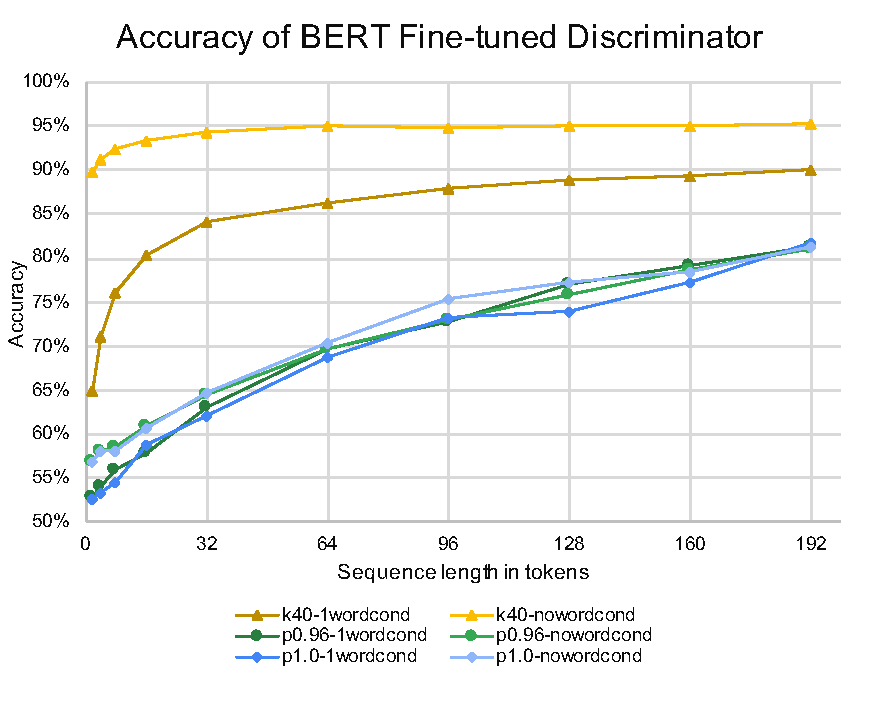
\includegraphics[width=\textwidth]{figures/bert_accuracy}
    \caption{}
    \label{fig:bert_accuracy} 
\end{subfigure}
\begin{subfigure}{.495\textwidth}
    \center
    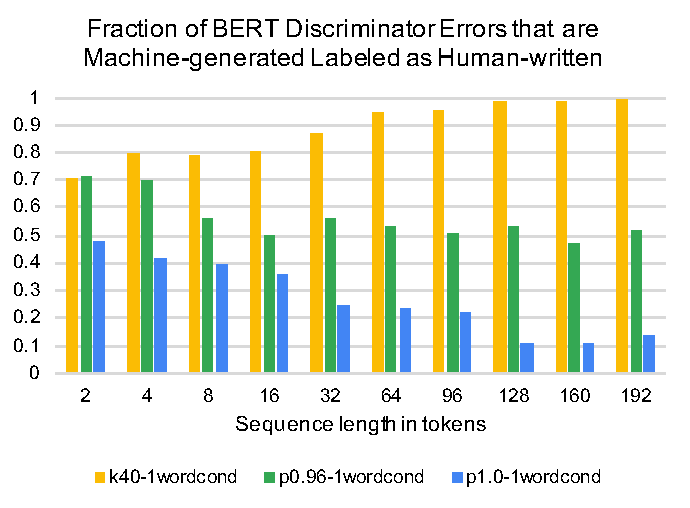
\includegraphics[width=\textwidth]{figures/fraction_incorrect_fp}
    \caption{}
    \label{fig:errors} 
\end{subfigure}
\caption{In \textbf{(a)}, accuracy increases as the length of the sequences used to train the discriminator is increased.
In \textbf{(b)}, we see that the BERT fine-tuned discriminator predicts about the same number of false-positives as false-negatives when trained with samples generated using top-$p$ sampling. However, for top-$k$, it more often mistakes machine-generated text to be human-written, while for untruncated random sampling the opposite is the case.}
\end{figure}

When generating with nucleus or untruncated random sampling, adding a priming token is not as impactful, as these methods are already sampling from a large fraction (or all) of the probability distribution.
This is seen in Figure \ref{fig:mean_ks} where at the very first step of unprimed generation, nucleus sampling selects from 3075 possible vocabulary words, and at later positions selects from on average more than 500.
Untruncated random sampling always selects from the entire 50,000 word vocabulary, whereas top-$k$ only selects from $k$.


\paragraph{Transferability}
In Table \ref{tab:transfer_accuracy}, we show how discriminators trained with samples from one decoding strategy can transfer at test time to detecting samples generated using a different decoding strategy.
Unsurprisingly a discriminator trained on top-$k$ generalizes poorly to other sampling methods: accuracy drops to as low as 42.5\%, \textit{worse than chance}.
Conversely, training the discriminator with sequences sampled from the untruncated distribution leads to little transferability to detecting top-$k$ samples.
Only the discriminator trained with nucleus sampling (a compromise between unmodified sampling and top-$k$) was able to detect sequences from the other sampling strategies without too much of a hit to accuracy.
As expected, a discriminator trained on an equal portion of data from each decoding method does reasonably at detecting all three.


\begin{table}[t]
  \small
  \centering
  \caption{Accuracy of BERT fine-tuned discriminator when trained on samples from one strategy (rows) and evaluated on another (columns). Trained on samples with 192 tokens. The `mixed' dataset is one containing an equal portion of samples from each strategy.}
  \label{tab:transfer_accuracy}
  \begin{tabular}{c c|c|c|c}
    \toprule
    & & \multicolumn{3}{c}{Eval} \\
    \cline{3-5}
    &            & top-$k$         & nucleus & random \\
    \hline
    \multirow{3}{0.7em}{\rotatebox[origin=c]{90}{\parbox[c]{1cm}{\centering Train}}} 
    & \multicolumn{1}{|c|}{top-k}   & \textbf{90.1} & 57.1          & 43.8 \\
    & \multicolumn{1}{|c|}{nucleus} & 79.1          & \textbf{81.3} & 78.4 \\
    & \multicolumn{1}{|c|}{random}  & 47.8          & 63.7          & \textbf{81.7} \\
    \hline
    & \multicolumn{1}{|c|}{mixed}  & 88.7          & 74.2          & 72.2 \\
    \bottomrule
  \end{tabular}
\end{table}

\begin{table}[t]
  \small
  \centering
  \caption{Average probability of `machine-generated' according to each length-192 discriminator. The expected in-domain probability is 0.5. One token of conditioning.}
  \label{tab:transfer-prediction}
  %                     p(machine)                              
  % dataset         k0-1wordcond k40-1wordcond p0.96-1wordcond
  % model                                                     
  % k0-1wordcond        0.382658      0.073189        0.226300
  % k40-1wordcond       0.145253      0.608884        0.278946
  % p0.96-1wordcond     0.488926      0.491959        0.517189
  \begin{tabular}{c c|c|c|c}
    \toprule
    & & \multicolumn{3}{c}{Eval} \\
    \cline{3-5}
    &            & top-$k$         & nucleus & random \\
    \hline
    \multirow{3}{0.7em}{\rotatebox[origin=c]{90}{\parbox[c]{1cm}{\centering Train}}} 
    & \multicolumn{1}{|c|}{top-k}   & 60.9 & 27.9 & 14.5 \\
    & \multicolumn{1}{|c|}{nucleus} & 49.2 & 51.7 & 48.9 \\
    & \multicolumn{1}{|c|}{random}  &  7.3 & 22.6 & 38.3 \\
    \bottomrule
  \end{tabular}
\end{table}

Perhaps this lack of transferability is related to each discriminator's calibration.
Indeed, the degree to which a discriminator's average prediction deviates from 50\% is a direct indicator of its accuracy. 
In Table~\ref{tab:transfer-prediction}, we observe that of the three BERT discriminators, only that trained on top-$p$ samples predicts `machine-generated' on approximately 50\% of in-domain examples as expected. 
This same discriminator's behavior holds on datasets generated by other sampling strategies as well. 
In contrast, we observe that discriminators trained on top-k and untruncated random samples severely underestimate the percentage of machine-generated excerpts in out-of-domain datasets.
Even within domain (Figure~\ref{fig:errors}), we find both discriminators heavily favor a single class, increasingly so as the number of tokens increases.

% False-negative = machine-written labeled as human-written
% Negative = machine-written
% Positive = human-written

\begin{table}
\setlength\tabcolsep{4.5pt}
    \small
    \centering
    \begin{tabular}{|p{0.40in}|p{0.42in}|p{0.35in}|p{0.35in}|p{0.35in}r|p{0.40in}|p{0.42in}|p{0.35in}|p{0.35in}|p{0.35in}r|}
\hline
\textbf{Truth} & \textbf{Raters} & \textbf{p1.0} & \textbf{k40} & \textbf{p0.96} & &
\textbf{Truth} & \textbf{Raters} & \textbf{p1.0} & \textbf{k40} & \textbf{p0.96} & \\
\hline
H & M & H & H & M & &
H & H & M & M & M & \\
\multicolumn{6}{|p{2.88in}|}{
\tiny
EDIT:OKAY!, I guess that'll work for now. \textgreater\_ http://www.teamfortress.com/ and then go buy the game and experience some of the best online gaming I have ever played. \textasciicircum\_\_\textasciicircum Both girls had a really fun time and I had a GREAT time making both of these costumes. Everything was altered even a little bit(dying the pants a darker grey and painting the boots and shirts) But my piece de resistance would have to be my eldest's Medi-Gun.If you have any questions about the costumes, I would be happy to assist you!Oh and here's a video of my daughter before the costume was completed.Thanks!
}&
\multicolumn{6}{p{3.03in}|}{
\tiny
Image copyright Getty Images Image caption Women mourn over the coffin of one of the victim's of Sunday's bombing in Ankara \textparagraph Who'd be in Turkey's shoes right now? \textparagraph Since July last year, hundreds of soldiers and civilians have been killed in terrorist attacks. Suicide bombs have torn into crowds of demonstrators and tourists. Military convoys have been targeted in the heart of the capital. \textparagraph A long-running Kurdish insurgency, once thought to be close to resolution after years of painstaking efforts to build bridges, has erupted once more. \textparagraph The country is awash with Syrian and other refugees. The government has been under pressure to stop them moving on into Europe and prevent would-be jihadis travelling the other way. \textparagraph How dangerous is Turkey's unrest? \textparagraph Tears and destruction amid PKK crackdown \textparagraph Turkey v Islamic State v the Kurds
}\\
\hline
\hline
\textbf{Truth} & \textbf{Raters} & \textbf{p1.0} & \textbf{k40} & \textbf{p0.96} & &
\textbf{Truth} & \textbf{Raters} & \textbf{p1.0} & \textbf{k40} & \textbf{p0.96} & \\
\hline
        M & M & H & - & - & &
        M & M & - & - & H & \\
\multicolumn{6}{|p{2.88in}|}{
\tiny
First off, this thread has done a pretty good job of describing in detail yet another broken touchscreen. That's the difference between a smartphone and a PC with no prying eyes having to snap shots for the police to find. \textparagraph What I would like to address is the mindset that generally surrounds Chrome OS users. To me this is analogous to saying that Apple does``hate their Windows", or that HP does``hate their Macs" as if http://twitter.com/) (and that quote is from two years ago), that anyone who covers smartphones and tablets from a ``PC" perspective is just jealous. \textparagraph Chrome OS is for browsing the web, PC processors can do stronger things in that regard, Windows is a juggernaut on those fronts. This is how I see it. Yes, it can be slow. And yes, you need a fast CPU
}
&
\multicolumn{6}{p{3.03in}|}{
\tiny
FOR ALABAMA, GOOD WEEKS \textparagraph AND A TOUR OF CAIRO \textparagraph THE ALABAMA COMMITTEE ON THE STUDY OF THE AMERICAN SECURITY AGENDA, \textparagraph America's future has been mapped out in carved stone. Metro Atlanta's last US congressman, Bill Posey, was a inextricable integral element of the Citadel project as it became another metaphor for Atlanta's transformation from an industry backwater into the finance and information hub of the nation's capital. Meanwhile, Cobb County -- Atlanta's geode of change -- is home to some of the largest industrial parks in the South, a regional cultural center, a 100-year-old manufacturing town and a potent symbol of the former city's cherished Georgian past. The gentry still live there, the defunct industrial landscapes carry the names of
}\\
\hline
\hline
\textbf{Truth} & \textbf{Raters} & \textbf{p1.0} & \textbf{k40} & \textbf{p0.96} & &
\textbf{Truth} & \textbf{Raters} & \textbf{p1.0} & \textbf{k40} & \textbf{p0.96} & \\
\hline
        M & H & - & - & M & &
        M & H & - & M & - & \\
\multicolumn{6}{|p{2.88in}|}{
\tiny
Exidentia at Eurnari, is an upcoming Cryptopia event which is currently still in development. Be a part of the first live stream of this year's event on 15-16 January 2016! \textparagraph Since the release of v1.22, Exidentia has received a fair amount of user feedback. This event takes place in the underwater Cryptopia they have built. During this event, you will learn about the ocean and areas around it, and be reached by a treasure hunter that helps you explore the different areas. \textparagraph There will be six different levels in this event that you will become acquainted with: thought Polar Lava, Ocean Seared Cones and Celestine Floors, Sea Damaged Aerie Bricks, coast Puddle (congipit stopping at red water), Shaikh Swamp and Bugmite. At rotating points, you will learn how to access various types of creatures
}
&
\multicolumn{6}{p{3.03in}|}{
\tiny
Ever since the opening of the North American College of Art Education in 1990, the demand for art education in America has grown steadily, and in recent years we have seen the rise of students that pursue art education not in the classroom but at art academies. This year saw another 50 percent increase in the number of art academies in the United States offering courses -- with an additional 10 percent of students in 2017 taking art. \textparagraph Some major changes have occurred in recent years with regard to the art curriculum and the way students learn, and we will explore each of these in coming months as we look at the various forms of art education. There is no one-size-fits-all approach for this or any other field of study, and students who begin a course in art education may change their plans based on what they see that course, including what lessons they have completed and the resources available, to create meaningful experiences of artistic creation. \textparagraph One important area
}\\
\hline

    \end{tabular}
    \caption{Some 192-token examples where at least two expert raters agreed with each other, but were not in agreement with the automatic discriminators. The first row shows examples where the ground-truth was human-written, the second shows machine-generated examples where the corresponding discriminator guessed incorrectly, and the third shows machine-generated examples where the discriminator was correct, but raters got it wrong.}
    \label{tab:qual_examples}
\end{table}

\paragraph{Human Accuracy}
Overall human performance across all sampling methods is shown in Figure \ref{fig:human_eval}b.
Even with the multi-paragraph 192-length excerpts, human performance is only at 71.4\%, indicating that even trained humans struggle to correctly identify machine-generated text over a quarter a time.
However, it is worth noting that our best raters achieved accuracy of 85\% or higher, suggesting that it is possible for humans to do very well at this task.
Further investigation is needed into how educational background, comfort with English, participation in more extensive training, and other factors can impact rater performance.

To break up the accuracies by sampling method in a way that is comparable to the results shown for the automatic discriminators, we pair each machine-generated example with a randomly selected one of webtext to create a balanced dataset for each sampling strategy.
Performance is shown in Figure \ref{fig:human_eval}a.
Top-$k$ produces the text that is hardest for raters to correctly distinguish, but as shown in Section \ref{section:auto_detection}, it is the easiest for our automatic detection systems.
Samples from untruncated random sampling and nucleus sampling with $p$=0.96 are equivalently difficult for raters to classify as machine-generated.
Our human evaluation results suggest that much lower $p$-values than the 0.92 to 0.98 range proposed in \citet{zellers2019defending} might be necessary in order to generate text that is considered significantly more human-like to human raters than the text produced by using the untruncated distribution.

Table \ref{tab:qual_examples} gives several examples where human raters and our BERT-based discriminators disagreed.
When raters incorrectly labeled human-written text as machine-generated, often the excerpts contained formatting failures introduced when the HTML was stripped out.
In the middle two examples, topic drift and falsehoods such as Atlanta being the ``information hub of the nation's capital" allowed humans to correctly detect the generated content.
However, in the bottom two examples, the high level of fluency left human raters fooled.

Overall we find that human raters---even ``expert" trained ones---have consistently worse accuracy than automatic discriminators for all decoding methods and excerpt lengths.
In our experiments, randomly-selected pairs of raters agree with each other on a mere 59\% of excerpts on average. (In comparison, raters and discriminators agree on 61\% to 70\% of excerpts depending on the discriminator considered).
We surmise that the gap between human and machine performance will only grow as researchers inevitably train bigger, better  detection models on larger amounts of training data.
While improved detection models are inevitible, it is unclear how to go about improving human performance.
GLTR proposes providing visual aids to humans to improve their performance at detecting generated-text, but it is unlikely that their histogram-based color-coding will continue to be effective as generative methods get better at producing high-quality text that lacks statistical anomalies.

% In this work, we study the behavior of automated discriminators and their ability to identify machine-generated and human-written texts. 
% We train these discriminators on balanced binary classification datasets where all machine-generated excerpts are drawn from the same generative model but with different decoding strategies.
% We find that, in general, discriminators transfer poorly between decoding strategies, but that training on a mix of data from methods can help.
% We also show the rate at which discriminator accuracy increases as excerpts are lengthened.
% 
% We further study the ability of expert human raters to perform the same task.
% We find that rater accuracy varies wildly, but has a median of 74\%, which is less than the accuracy of our best-performing discriminator.
%Most interestingly, we find that human raters and discriminators make decisions based on different qualities, with humans more easily noticing semantic errors and discriminators picking up on statistical artifacts.
% In our experiments, these artifacts are most prominent with top-$k$ sampling.
%However, any strategy that over-samples high-likelihood words is susceptible.
%As the $p$ in nucleus sampling is set increasingly lower to achieve more fluent text (some systems are already using $p$ as low as 0.5 \citep{miculicich2019selecting}), the distributional deviations that plague top-$k$ text will surface in nucleus sampling as well.

%\citet{holtzman2019curious} explain how a unique attribute of human language is that it dips in and out of low probability zones.
%This variance in likelihood is what makes human-written text interesting and exciting to read.
%Today's generation systems have not yet solved the problem of mimicking the human cadence without introducing poor word choices that are easy for humans to detect. 
%Generation systems often optimize for fooling humans without acknowledging the trade-off that exists between human perception of quality and ease of automatic detection.
%We therefore suggest three prongs for future research:


% \section{Detecting the Boundary between Human-Written and Machine-Generated Text}
\section{\ROFT: A Largescale Study of Human Detection Ability}
\label{section:roft}

Our pilot study in Section \ref{section:detection} showed how choice of decoding strategy impacts human ability to detect machine-generated text.
However, there are many other factors which influence detectability that we were not able to include in this study, including the domain of the text being used for evaluation and the architecture and manner in which the underlying language model was trained.
In addition, we were interested in studying the annoators themselves--how do annotator background as well as the incentive structure set up for soliciting annotations impact performance on the detection task?
We therefore saw the necessity of designing a platform for conducting large-scale studies of the detection task.

Previous studies, including our pilot, focused on the binary classification task--given a text example that is either entirely human-written or entirely machine-generated (aside from an initial prompt), annotators must predict whether it is human-written or machine-generated.
For example, \citet{clark2021all} demonstrated that annotators are able to distinguish GPT-2 XL generations with at best 62\% accuracy, but they perform no better than random chance on GPT-3 outputs \citep{brown2020language}.
Even after training evaluators to improve their detection abilities, detection accuracy on GPT-3 was only able to converge to around 55\%.
An older study by \citet{brown2020language} reported similarly low performance (52\%) on the detection of machine-generated news articles.

For our large-scale study, we instead framed detection as a boundary-detection task: given a document that starts off as human-written and at some point transitions to machine-generated, can annotators detect the transition point?
The boundary detection setting is more informative than the classification setting because it better aligns with how LMs are used to generate text in practice; in typical usage, a generative system is provided with a prompt and asked to produce a continuation.
By measuring human skill at the boundary detection task, we were able to evaluate the relative performance of different generative systems, build a better understanding of how incentive structure influences the quality of the annotations acquired, and make progress toward quantifying the risks associated with large language model goals..
Furthermore, because the annotation platform we built was public, we could achieve these research goals while simultaneously educating the public about how to spot generated text. 

In total, we collected over 20,000 annotations with the goal of answering the following research questions:
\begin{itemize}[itemsep=0.5pt,topsep=1pt]
    \item How do model size, decoding strategy, and prompt genre impact dectability?
    \item What kinds of errors and textual properties do humans associate with machine-generated text?
    \item Do annotators who take longer per annotation or spend more time on the task do better?
    \item Are their external factors (such as knowledge of NLG) which make some annotators better at the task?
\end{itemize}

\begin{figure}[t]
    \centering
    \framebox{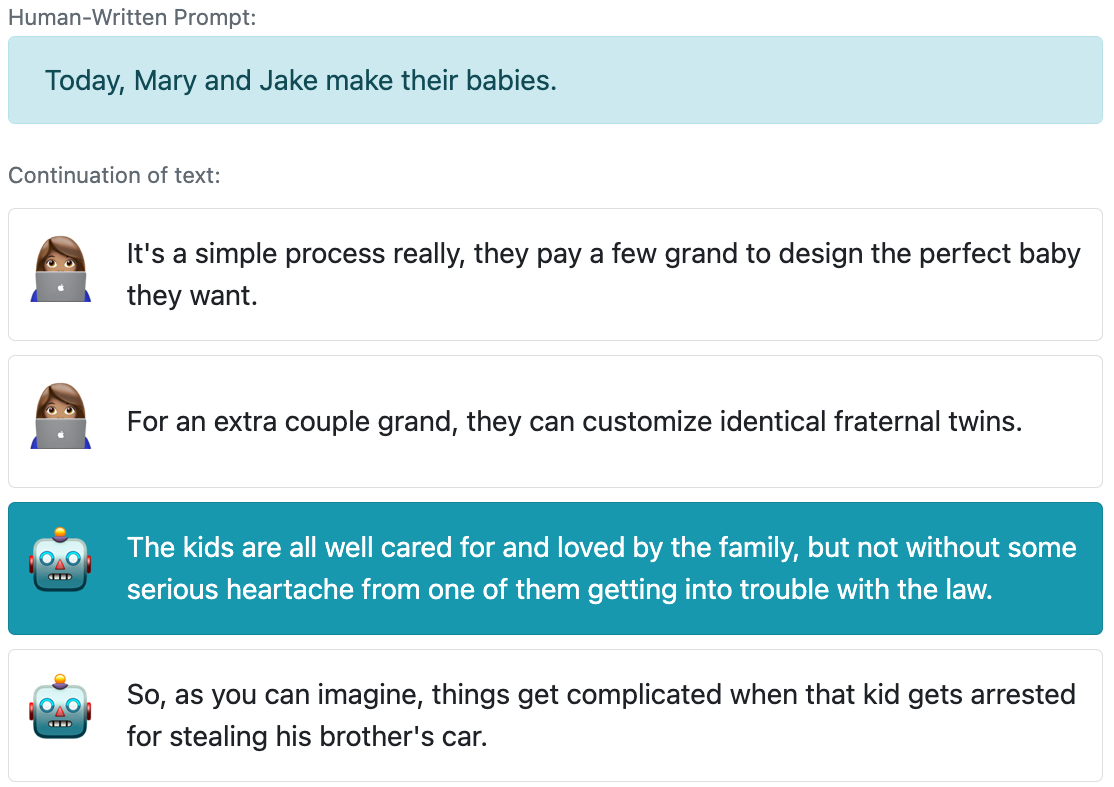
\includegraphics[scale=0.3]{figures/interface.png}}
    \caption{In the boundary detection task, players see one sentence as a time and try to guess when they transition from human-written to machine-generated.}
    \label{fig:pg1}
\end{figure}

% \subsection{Related Work}

% Another related area of research is asking annotators to explain why they think generated text is generated.
% \citet{he2021tgea} created a dataset of generated text annotated with the errors that humans found in it, and \citet{dou2021scarecrow} proposed an error annotation schema for generated text.
% The errors we allow players to report in our experiments were inspired by this schema.

% In this paper, we expand on the findings of previous research by altering the evaluation methodology from a classification task over an entire text to a boundary detection task, where human evaluators are asked to identify the sentence at which a passage transitions from being human-written to machine generated. We also display the effect of annotator ``training'', where we investigate whether repeated attempts at the task with feedback yields better performance over time. We provide additional insight into detection performance, by controlling for variables such as hyperparameter value, model parameter size, and textual domains.

\subsection{The Real or Fake Text Game}
Our study uses data collected through the ``Real or Fake Text'' (\ROFT{}) annotation platform \citep{dugan2020roft}.
\ROFT{} is a turn-based game where a player first selects a domain of text (news articles, recipes, short stories, or speeches).
The player then plays a series of game rounds.
Figure \ref{fig:pg1} shows a screenshot from a game round.
In each round, the player is shown a starting sentence which they are told comes from a real human-written document.
They are then shown subsequent sentences, one at a time.
Each subsequent sentence may be the true continuation of the document, or it may be text generated by a language model.
Once the sentences transition to being machine-generated, they will stay so for the rest of the 10-sentence passage.

After being shown each sentence, the player must guess whether that sentence was machine-generated or human-written.
If the user selects ``human-written,'' another sentence is displayed.
If the player deems the current sentence to be written by a machine, the game round ends and the true author (machine or human) for each sentence is revealed, potneitally allowing the player to improve their intuitions over time.
Before submitting their selection, the player is able to select a reason to explain their choice of sentence.
They may select from a pre-defined set of reasons (Table \ref{tab:reasons_text}) or else write a custom reason.
Thus, the player's goal in \ROFT{} is to correctly identify the sentence at which a passage transitions from being human written to being generated by a language model.
This setting is considerably more realistic than prior work, since in the real world, generating with a prompt is the standard way to achieve controllability, and malicious actors will not reveal what portion of a generation is the human-written prompt.

In total we collected over 20,000 annotations.
We found that players vary substantially in their detection ability, and that factors such as the amount of time taken to complete a game round and total number of game rounds played sometimes correlate with success.
Furthermore, we examine some of the the trends and errors which distinguish real from generated text and look at whether annotators could pick up on these trends.
Finally, we discuss the difficulty in incentivizing players to improve in their ability over time.

\subsection{Experimental Design}

\subsubsection{Datasets}
In order to answer questions of how textual genre and writing style affect detectability of machine-generated text, we selected four diverse categories of prompts. 
For each category, documents were sentence-segmented, and only documents with 11 or more sentences were retained.
For each document, the first $h$ sentences were used as the prompt, where $h$ is a uniform random number between 1 and 10 (inclusive). The remaining $10-h$ sentences of each 10-sentence game round were a machine-generated continuation. Our four genres of prompts are as follows:

\paragraph{News articles.}
Documents were drawn from the New York Times Annotated Corpus \citep{sandhaus2008new}, which contains 1.8 million articles published by the Times between 1987 and 2007.
Our hypothesis was that this domain would be challenging for models since news requires factual accuracy, which state of the art models have been shown to struggle with \cite{nakano2021webgpt, lin2021truthfulqa}. 

\paragraph{Presidential speeches.}
Documents were drawn from the presidential speech corpus \citep{brown2016cops}, which contains 963 speeches given by presidents of the United States, with dates ranging from 1789 to 2015.
Our hypothesis was that the sort of first-person rhetoric found in these speeches would be easy for models to impersonate since political speech and first-person speech are plentiful in web-based training data.

\paragraph{Stories.}
Fictional stories were selected from the Reddit Writing Prompts dataset \citep{fan2018hierarchical}, a corpus of amateur short stories scraped from the r/WritingPrompts sub-Reddit.
We hypothesized that this domain would be challenging for players since the writing quality of the stories is not especially high (which lowers the bar for the model generation quality), and factuality is not as important in a fictional domain.

\paragraph{Recipes.}
Recipes were extracted from the Recipe1M+ dataset \cite{marin2019learning}.
Recipes were parsed slightly differently than the other domains.
We set the ``first sentence'' of each document as the name of the recipe and the ingredient list, and each subsequent ``sentence'' was a step in the recipe. Some recipe steps were more than one sentence. We hypothesized that this dataset would be difficult for models due to the closed-ended nature of the task and the reliance on common sense. 

\subsubsection{Awarding Points}
\label{sec:points}
In each game round, the player is awarded points based on how close their selection was to the true boundary\footnote{For our purposes, the ``boundary'' sentence is considered to be the first machine-generated sentence in the passage}.
Players were awarded 5 points for correctly choosing the boundary sentence and $\max(5-n, 0)$ points for a guess $n$ sentences after the boundary.
Players were not awarded points for guessing a sentence before the boundary.
Players were able to see how many points they earned in each category on their profile page and compare their performance with fellow players on the leaderboard page.
In the Findings section (Section \ref{section:roft_results}), we report mean score earned as the predominant evaluation metric. 
Table \ref{tab:correlations_with_other_metrucs} shows the correlation between mean score and other sensible metrics.
We see that mean score is strongly positively correlated with both perfect guess accuracy and correct side of boundary. Mean score is only weakly correlated with distance after boundary due to the harsh scaling of points; only guesses within five sentences to the right of the boundary receive any points. While imperfect, this harsh scaling is by design, as without it later sentences will give significantly more points in expectation.

% Users are additionally given profiles, and are able to collect "trophies" for various accomplishments during the annotation task (e.g. getting the boundary exactly correct) in a manner to incentivize additional annotation collection.

\subsubsection{Player Recruitment and Annotation Filtering}
\label{sec:players}
Players were recruited from two sections of an Artificial Intelligence course for Master's students and senior undergraduates at the University of Pennsylvania.
We only analyze fully anonymized data from students who consented to having their annotations used for research purposes.

% TODO: Replace with University of Pennsylvania after anonymity period.
The first section (Group A) was asked to play 30 minutes of the \ROFT{} annotation game for a fixed amount of points of class credit.
Students in this section were not given any instructions beyond how to create an account.
The second section (Group B) was explicitly told they would be awarded to 2 points of extra credit toward their final grade.
The amount awarded was $\min(2p/250, 2)$ where $p$ was the number of points the student earned on the \ROFT{} leaderboard.
Students in Group B were given detailed instructions and examples of signs to look out for that text was machine-generated.
% TODO: Change google doc to be PDF and host on roft cloud bucket
Table \ref{tab:particpants} gives statistics on the annotations collected from each class.

We note that university students taking an advanced artificial intelligence course are not reflective of the global population of English speakers, and the results presented in this paper may not reflect the general population's ability to detect machine-generated text. 

In total, we collected 42,165 annotations over 7,895 different game rounds.
The annotations were then filtered in the following ways.
If a player guessed the same boundary position for a series of 5 or more rounds in a row, we removed all the annotations in the series because the player was likely no longer actually playing the game as designed.
We also removed annotations from the two players cheated by exploiting Javascript vulnerabilities.
Finally, for the recipes genre, a bug during dataset curation resulted in an over-representation of ``all-human'' game rounds played;
for better balance during analysis, we randomly removed a portion of these annotations.
Our final filtered dataset consisted of 21,646 annotations over 7,257 game rounds.
For News, Stories, and Recipes, we had on average over 2 annotations per game round, while for Speeches, a smaller dataset, we had on average 16.
Table \ref{tab:dataset_stats} gives a detailed breakdown of the dataset across genres and generation systems.


\begin{table}[tb]
\center
\small
\caption{Statistics on the annotation tasks (game rounds) available in our system. The second column shows the number of game rounds available for each system. The discrepancies in number of annotations per dataset is partially due to the fact that players were able to choose which domain they performed annotations in.}
\label{tab:dataset_stats}
	\begin{tabular}{l|r|rr|r|p{2in}|p{1.5in}}
\toprule
 & \# & \multicolumn{2}{|c|}{\# Annotations} & {Avg} & & \\
Genre & Rounds & Raw & Final & Ann/Gen & Systems & Decoding Strategies \\
\midrule
News & 1,838 & 7,806 & 4,488 & 2.97 &
\begin{minipage}{.275\textwidth}
      
\includegraphics[height=1em]{figures/model_dist_new_york_times}
\end{minipage}
&
\begin{minipage}{.225\textwidth}
      
\includegraphics[height=1em]{figures/decoding_dist_new_york_times}
\end{minipage}
\\
Stories & 9,864 & 8,007 & 4,614 & 2.53 &
\begin{minipage}{.275\textwidth}
      
\includegraphics[height=1em]{figures/model_dist_short_stories}
\end{minipage}
&
\begin{minipage}{.225\textwidth}
      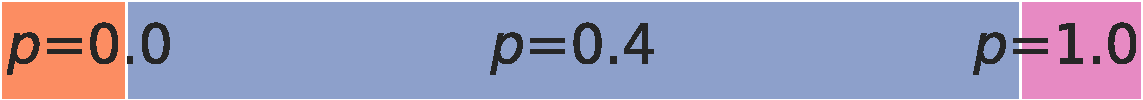
\includegraphics[height=1em]{figures/decoding_dist_short_stories}
\end{minipage}
\\
Recipes & 7,258 & 17,978 & 7,709 & 2.13 &
\begin{minipage}{.275\textwidth}
      
\includegraphics[height=1em]{figures/model_dist_recipes}
\end{minipage}
&
\begin{minipage}{.225\textwidth}
      
\includegraphics[height=1em]{figures/decoding_dist_recipes}
\end{minipage}
\\
Speeches & 297 & 8,374 & 4,835 & 16.28 &
\begin{minipage}{.275\textwidth}
      
\includegraphics[height=1em]{figures/model_dist_presidential_speeches}
\end{minipage}
&
\begin{minipage}{.225\textwidth}
      
\includegraphics[height=1em]{figures/decoding_dist_presidential_speeches}
\end{minipage}
\\
\bottomrule
\end{tabular}
\end{table}

\begin{table}[tb]
\center
\small
\caption{Statistics on the students who were invited to complete annotations on \ROFT. ``Avg Ann / Part'' is the average number of annotations per participating student,  while ``Avg Score / Part'' is the average score. ``Avg Time'' is the average time it took a participant to read one sentence. Standard error is shown.
}
\label{tab:particpants}
\begin{tabular}{l|rrrrr}
\toprule
      & \#              &                & Avg Annotations & Avg Score     & Avg Time /\\
Class & \# Participants & \# Annotations & / Participant   & / Participant & Annotation (s)\\
\midrule
Group A & 141 & 6,527 & 46 & 1.966 & {5.651} \\
Group B & 102 & 15,119 & 148 & 2.134 & {6.443} \\
\midrule
Overall & 241 & 21,646 & 90 & 2.083 & {6.338} \\
\bottomrule
\end{tabular}
\end{table}

\subsubsection{Continuation Sources}

In order to answer questions related to how model attributes affect generated text we employed different methods of text generation for each category.
For Recipes, New York Times, and Stories, we generated continuations with GPT-2 XL using nucleus sampling \citep{holtzmanetal2020} with $p=0.4$ and a repetition penalty of $1.2$ \citep{keskar2019ctrl}.
For Recipes, we additionally generated continuations with a GPT-2 XL model finetuned on recipes.

For New York Times and Stories, we experimented with varying the $p$ used for decoding, testing out $p=0.0$ (argmax) and $p=1.0$ (sampling directly from the model's predicted distribution).
As an additional sanity check on annotator skill, we also included 100 game rounds in the News domain where instead of transitioning to an LM-generated continuation, the passage transitioned to a completely different news article selected at random.
We expected these game rounds to be trivial for players.

% For New York Times, we also added 100 attention-check game rounds (10 for each possible context length), where rather than transitioning to machine-generated text, the passage transitioned to sentences from a randomly selected news article.
% We refer to this as the ``random'' model in our analysis and expect these game rounds to be trivial for players.

For Stories, we experimented with different model sizes, generating continuations with both GPT-2 Small (117M Parameters) and GPT-2 XL (1.5B Parameters).
Lastly, for Presidential Speeches, we generated continuations using the CTRL model \citep{keskar2019ctrl} rather than GPT-2.
CTRL has the option to specify a control code indicating what domain to generate text in. For half of the generations, we used the ``[Politics]'' control code while for the other half we randomly selected a control code each time.
We expected use of the politics control code to result in generations which more on topic.

Table \ref{tab:dataset_stats} gives the statistics of the game rounds included in \ROFT{}.
Overall, \TODO{}\% of game rounds were exclusively human-written.





\begin{table}
    \centering
    \small
    \begin{tabular}{c|c}
    \toprule
    Metric & $\rho$ \\
    \midrule
    (a) Correct side of boundary &  0.74 \\
    (b) Perfect guess & 0.88 \\
    (c) Distance after boundary & 0.31  \\
    \bottomrule
    \end{tabular}
    \caption{Average points earned is the main metric reported in the Results section. This table shows the Spearman's rank correlation between average points per user and several other possible metrics: (a) the fraction of times the user correctly guessed on or after the boundary; (b) the fraction of times the user guessed exactly on the boundary; and (c) the average number of sentences after the boundary of the user's guess (giving new score for guesses before the boundary).}
    \label{tab:correlations_with_other_metrucs}
\end{table}

\subsection{Results}
\label{section:roft_results}
The collected annotations allow us to investigate several questions.
Error bars on all figures and tables are 95\% confidence intervals.

\subsubsection{Can humans detect generated text?}
Players correctly guessed exactly on the boundary sentence 23.4\% of the time.
For game rounds which contained at least one generated sentence, players were able to eventually guess machine-generated 72.3\% of the time, even if they missed the exact boundary. % TODO (Daphne) does this mean predicted >= true && true != 9 ?
Players incorrectly identified 61.3\% of all-human game rounds as containing machine-generated text.

The average number of points (\S\ref{sec:points}) received per round by our players was 2.08, well above random chance.
For comparison, if a player uniform randomly guessed every round, their expected per-round score would be 1.31, and
if they always guessed the last sentence, their expected per-round score would be 1.5.\footnote{These expectations assume that the true boundary position is equally likely to be at any position. Figure \ref{fig:distribution_true_boundaries} shows the true distribution of boundaries, which was not quite uniform.}
For the remaining analyses, we will use average points earned as the primary measure of detection ability.
This measure correlates with other possible metrics (Table \ref{tab:correlations_with_other_metrucs}).

Out of the 214 annotations we collected on the ``sanity check'' game rounds, the mean score was 2.75, significantly higher than any of the true LM-backed systems.
Also, for these annotations, the error type ``irrelevant'' was selected about twice as often as all other error types combined, validating that players were paying attention to the task at hand.

\begin{figure}
    \centering
    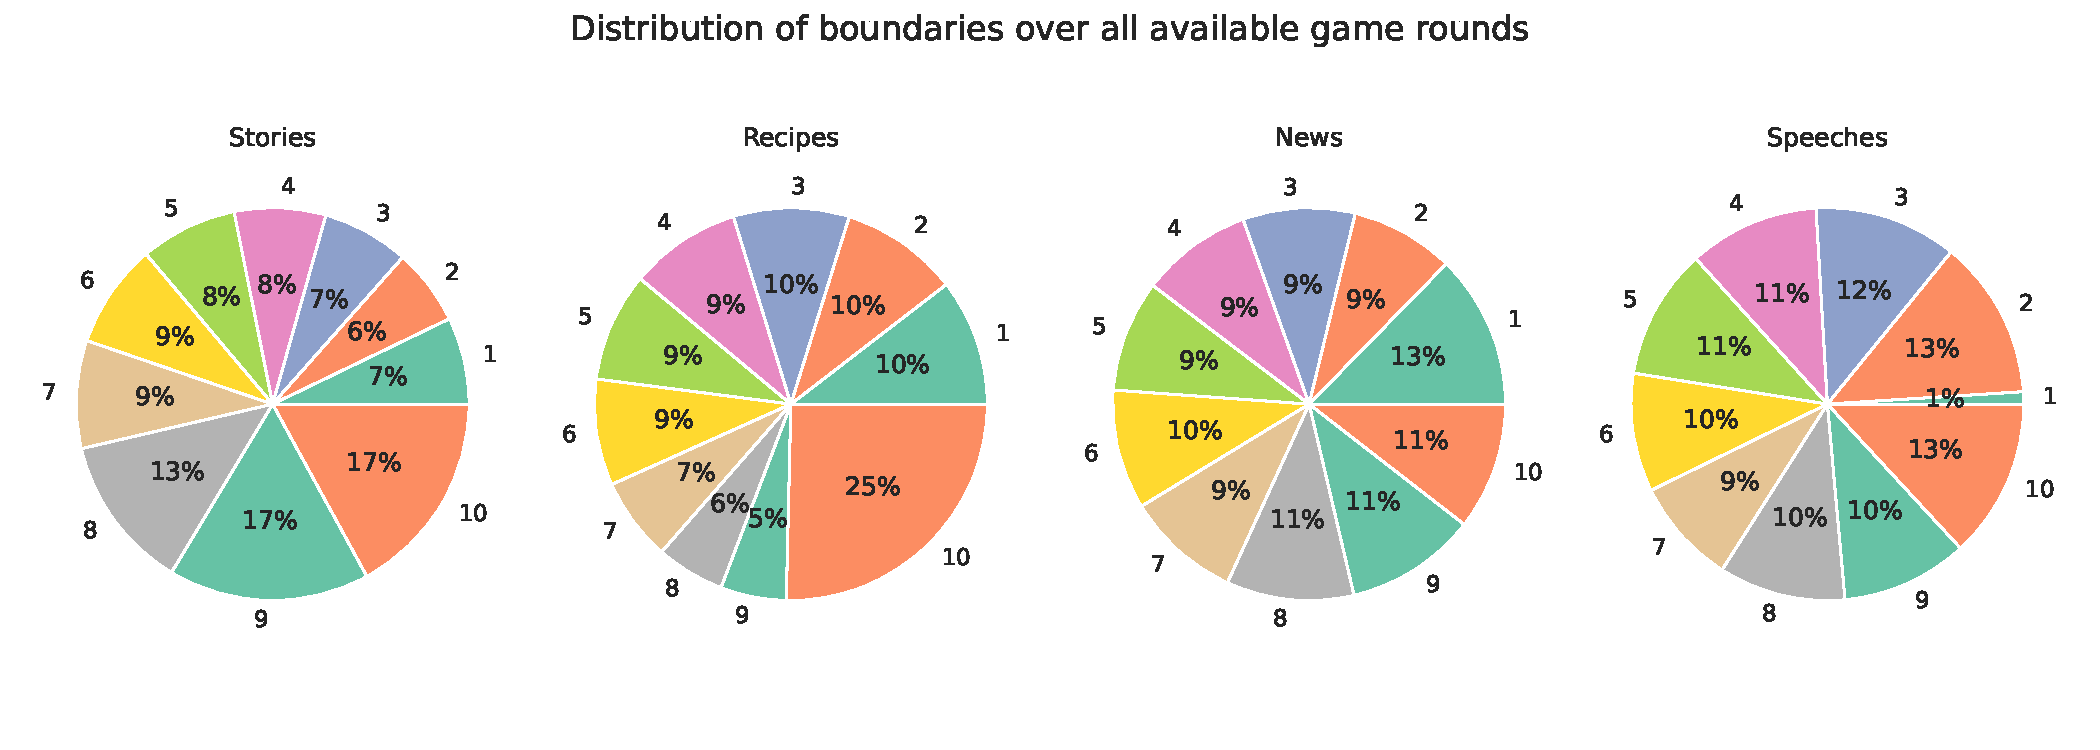
\includegraphics[width=0.8\linewidth]{figures/available_game_rounds.pdf}
    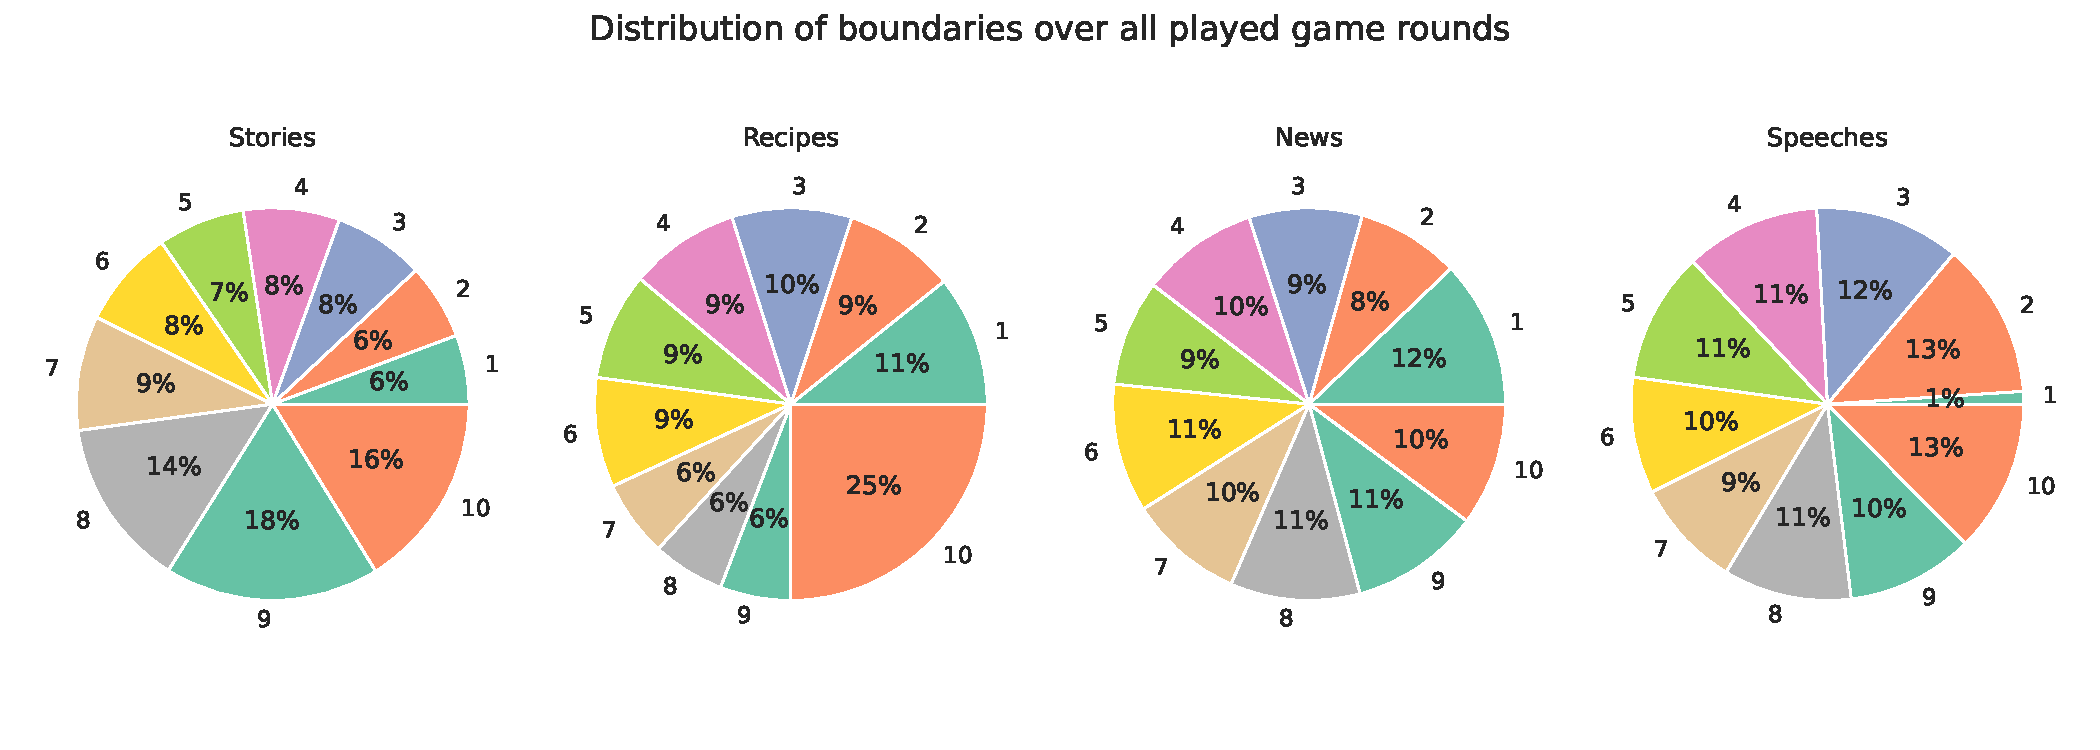
\includegraphics[width=0.8\linewidth]{figures/played_game_rounds.pdf}
    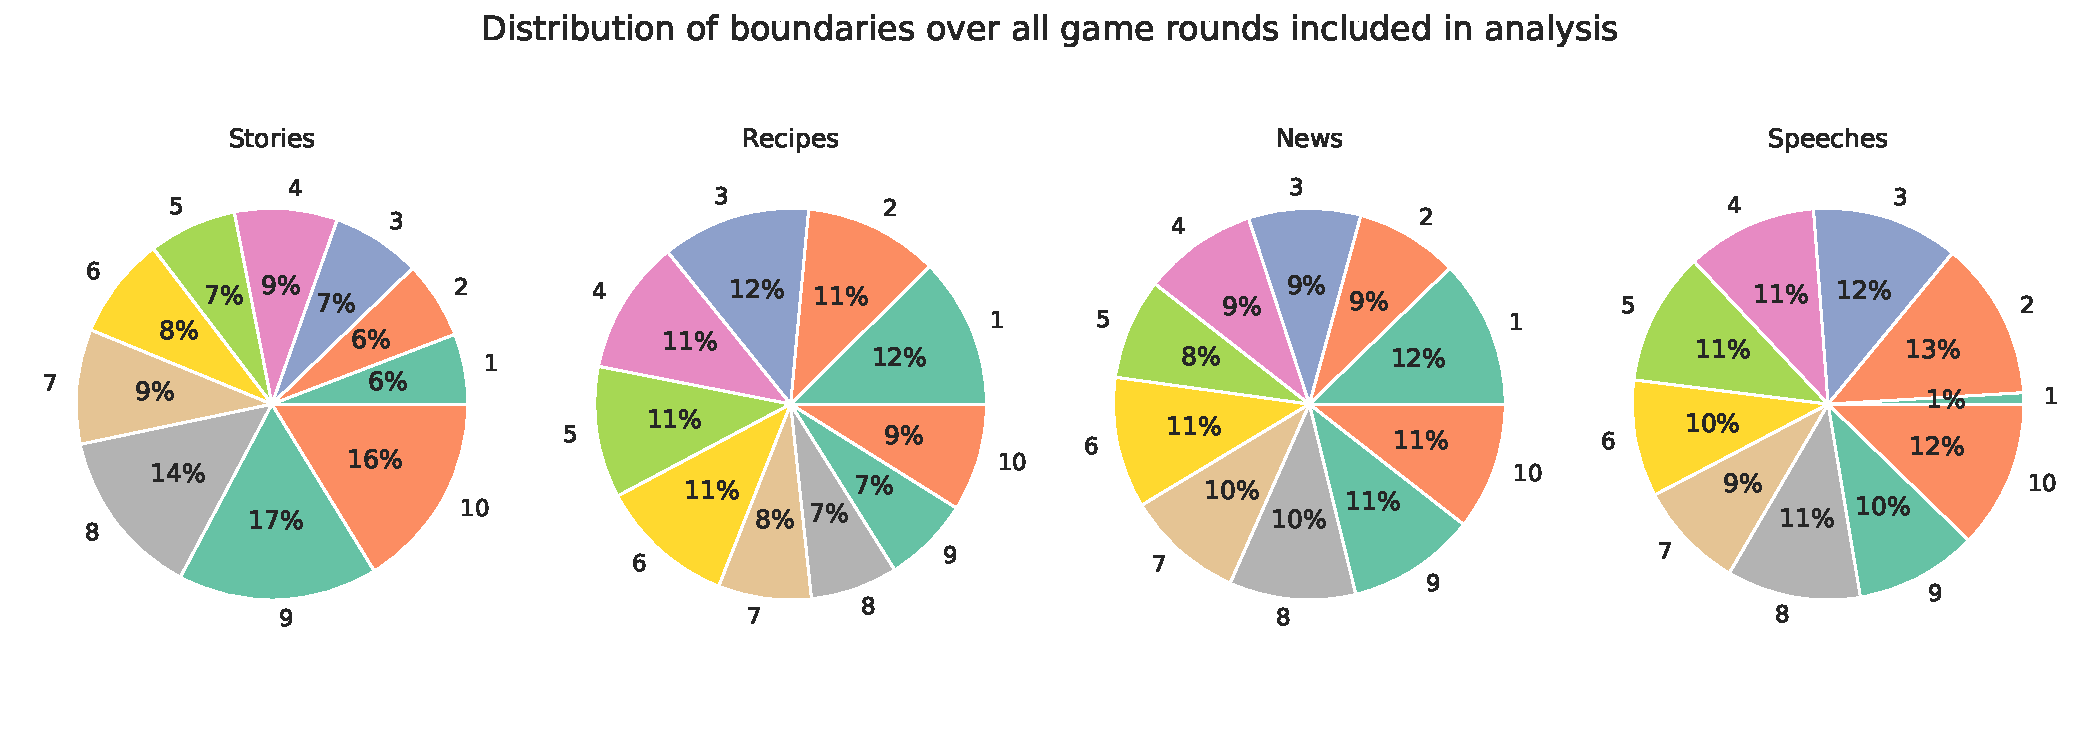
\includegraphics[width=0.8\linewidth]{figures/analyzed_game_rounds.pdf}
    \caption{The distribution of boundary sentence positions over all game rounds available on RoFt (top), all game rounds that received annotations (middle), and all game rounds included in this paper's analysis after filtering out problematic annotations (bottom).}
    \label{fig:distribution_true_boundaries}
\end{figure}

\subsubsection{How much does player ability vary?}
There was a large variance in the skill of individual players.
Out of the 116 players who completed 50 game rounds, 19 earned a total score of 70 or fewer points (one std below the mean score) in their first 50 rounds, while 15 earned a total score 127 or greater points (one standard deviation above the mean score). Four of these raters scored two standard deviations above the mean score.

We also found that under the right conditions, players can improve over time.
There was no correlation between number of rounds played and player score for Group A.
However, Group B, who were given extra credit proportional to their game score, did show slight improvement (Table \ref{tab:correlation_over_time}). 
There was also lower variance in points earned among students in Group B (Figure \ref{fig:skill_over_time}), possibly because they were more incentivized to do well at the task.

% We hypothesize that the difference between these two group comes from better guidance as to what to look for in generated text and more performance-based incentives to improve at the task.

% Given the tendency for annotators to game our system by learning to select all sentences as human-written, we hypothesized that this improvement over time may actually be attributable to annotators learning how to maximize points rather than actually improving at the detection task. To combat this, we re-conducted our analysis with much more aggressive filtering and got similar results. A more detailed reporting of this experiment can be found in Appendix \ref{app:gaming}.

We can also measure inter-annotator agreement with the Krippendorff's alpha co-efficient.
This statistic measures how much disagreement there is between players compared to the amount of disagreement one would expect by chance.
Two players are considered to have agreed if they both guessed ``machine-generated'' on any sentence after the true boundary or if they both guessed the entire passage was human-written.
Over all annotations, we found $\alpha$=-0.25, indicating there was less agreement than could be expected from random guessing, suggesting different annotators were better at identifying different kinds of problems with LM-generated text.
However, among our top 25\% of players (measured by mean score), there was high inter-annotator agreement, with  $\alpha$=0.44, suggesting that good annotators made similar errors.

\begin{figure}[tb]
    \centering
    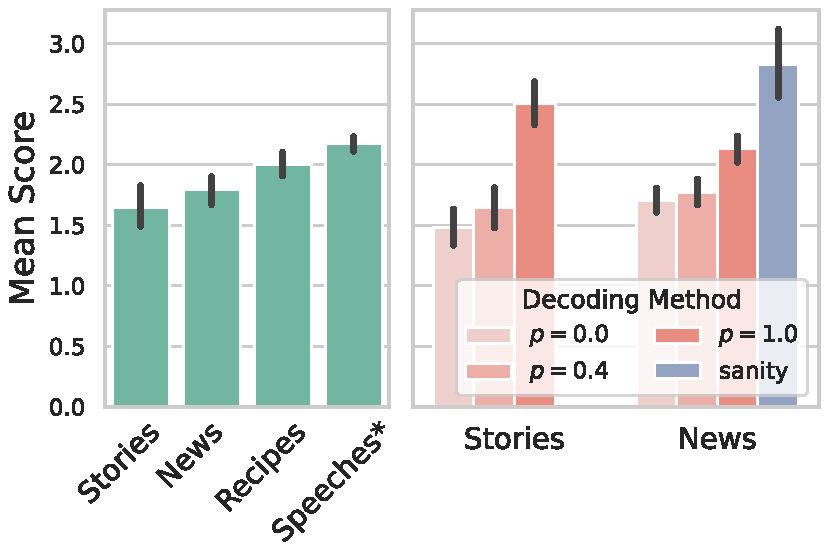
\includegraphics[width=0.5\linewidth]{figures/domain_topp.pdf}
    \caption{\textbf{(left)} Comparison of mean player score across different genres with GPT-2 XL $p$=0.4 (and CTRL $p$=0.4 for speeches). \textbf{(right)} Comparison of mean player score across different values of $p$ for nucleus sampling (GPT-2 XL), as well as a ``sanity-check'' baseline.}
    \label{fig:genre_top_p}
\end{figure}

\begin{figure}[tb]
    \centering
    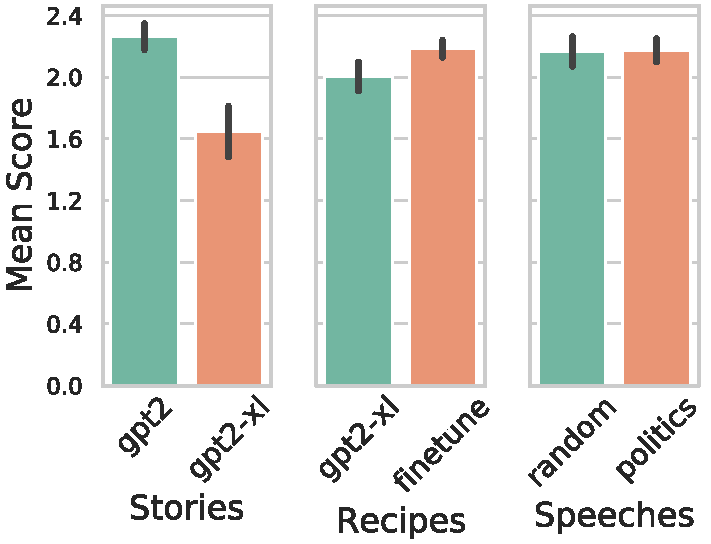
\includegraphics[width=0.4\linewidth]{figures/model_size_and_finetuning.pdf}
    \caption{\textbf{(left)} For Stories, as model size increases (using $p$=0.4), detection becomes harder. \textbf{(middle)} For Recipes, extra finetuning does not significantly impact detectability. \textbf{(right)} For Speeches, using a ``[Politics]'' control code (with the CTRL model) has no impact on detectability compared to using a random control code.}
    \label{fig:model_size_finetuning}
\end{figure}

\subsection{Analysis}

\subsubsection{Are some genres easier to detect?}
We found that generated text was easier to identify in the recipes and speeches genres than in the stories and news genres.
Figure \ref{fig:genre_top_p} (left) shows the average points received on each genre for game rounds that used comparable LMs, while Table \ref{tab:scores_per_domain} gives a more detailed breakdown across models. 

For recipes, we expect that the task was made easier by the fact that the first human-written "sentence" in each game round was a semi-structured ingredients list, making it easy for players to check for contradictions---a step saying to mix in cream is probably generated if there is no cream ingredient.
In addition, recipes often assume implicit unwritten knowledge, which language models struggle to get right---a step saying to crack eggs into a bowl must precede a step saying to  whisk the eggs.
Indeed, if we look at the reasons given by our players for saying ``machine-generated,'' recipes had a much larger percentage of ``common\_sense'' errors (26\%) than did either News (10\%) or Stories (10\%).
It is worth noting that this result slightly contradicts the one reported by \citet{clark2021all} who reported that generated recipes were more difficult to detect than news or stories; more targeted research is necessary to fully understand the relationship between domain and generation performance.

We believe the speech genre was easier for players not because speeches are intrinsically more difficult to generate but because we struggled to get the CTRL model to produce high-quality, non-repetitive generations, even though it is about the same size model as GPT-2 XL.
It was necessary to incorporate repetition penalties during generation with CTRL, which helped but did not
solve the quality issues.

\begin{table}
\small
\begin{center}
\begin{tabular}{S|SSS} \toprule
    {Dataset} & {$p$} & {$n$} & {Mean Score}\\ \midrule
    {News} & {0.4} & {1,197} & {1.793$\pm$0.109} \\
    {Stories} & {0.4} & {468} & {1.645$\pm$0.168} \\
    {Speeches*} & {0.4} & {4,252} & {2.171$\pm$0.062}\\
    {Recipes} & {0.4} & {1,811} & {2.004$\pm$0.098} \\
    \bottomrule
\end{tabular}
\caption{The mean scores for each domain on annotations involving XL-sized models for $p$=0.4. Asterisk denotes generation by CTRL. Interval is $\alpha=0.95$ confidence.}
\label{tab:scores_per_domain}
\end{center}
\end{table}

\subsubsection{Does model size make a difference?}
Previous work has shown that language model performance scales with number of parameters \citep{kaplan2020scaling}, so we expected players to be worse at detecting generations from larger models.
Indeed, we found that players scored significantly higher when generations came from GPT-2 small (117M parameters) than when they came from GPT-2 XL (1.5B parameters) (Figure \ref{fig:model_size_finetuning}.).

% We additionally experimented with the GPT-3 Davinci model (150B parameters) but were unable to collect enough annotations to draw any statistically significant conclusions.


\subsubsection{Are diverse generations easier to detect?}
Choice of decoding strategy is known to have significant impact on text quality \citep{zhang2021trading} and detectability \citep{ippolito2020automatic}.
Choosing a lower value of $p$ when generating with a nucleus sampling \citep{holtzman2019curious} decoding strategy produces less diverse but also less noisy text than choosing a higher value of $p$.
In our experiments, we did not find statistically significant differences in player skill between $p$=0.0 (greedy) and $p$=0.4 sampling (Figure \ref{fig:genre_top_p}).
However, players were significantly better at $p$=1 (pure random sampling) than the lower values, 
validating claims from earlier papers that LMs struggle to generate high-quality text with similar diversity to human-written text.
Interestingly, generations from GPT-XL using $p$=1.0 were easier for players to detect than generations from GPT-2 small using $p$=0.4.
This highlights the importance of decoding, as improper selection of decoding strategy may cause a language model to perform worse than one that is one tenth its size.
% This further emphasizes the need for automatic detection tools to be used alongside human players in the boundary detection task as well as the binary detection task.
% maybe mention the differences in reasons given for different p values. mention how the GROVER paper says that human text's perplexity is more similar to p=0.92 (lol)


\subsubsection{Do control codes affect detectability?}
CTRL is a 1.6B parameter LM trained with controllability in mind.
At inference time, one can pass in a control code, such as ``[Politics]'' or ``[Horror]'' to include the style of the generated text.
We investigated the efficacy of these control codes on the genre of presidential speeches by using ``[Politics]'' for half the generations and randomly selecting control codes for the remaining half.
We found that use of the politics control code did not significantly affect  players' ability to distinguish real from fake text.
This is not to say that control codes do not affect generation; however, it does suggest that the cues used by players to detect generations may not be related to genre-specific details, as least not within the genre of political speeches.
Further work is needed to investigate whether control codes could have influenced detectability in other genres.

\subsubsection{Does finetuning affect detectability?}
We had expected that finetuning on in-domain text would result in a model that was better able to fool humans.
Counter to expectations, there was a small increase in player detection ability when generations came from GPT-2 finetuned on recipes compared with generations from pre-trained GPT-2. This is despite the fact that the finetuned model had close to half the perplexity of the pre-trained model on a held out test set of 50,000 recipes (4.781 vs. 8.979).
While we can only speculate as to the amount of recipe knowledge present in the pre-trained model (GPT-2's training data is not publicly available), it is possible the pre-trained model already contained enough understanding of recipe-like text that it was not critical to do the extra-finetuning.
Perhaps finetuning would have had more impact in a specialized or jargon-laden domain (e.g. legal, medical).


% However, it may also be the case that a sufficiently long prompt is enough priming to put any vanilla model with broad enough training data into a space where it generates comparative to a finetuned model. Future work should seek to further investigate this area and determine how finetuning may affect both automatic and human detection accuracy.

\begin{figure}[tb]
    \centering
    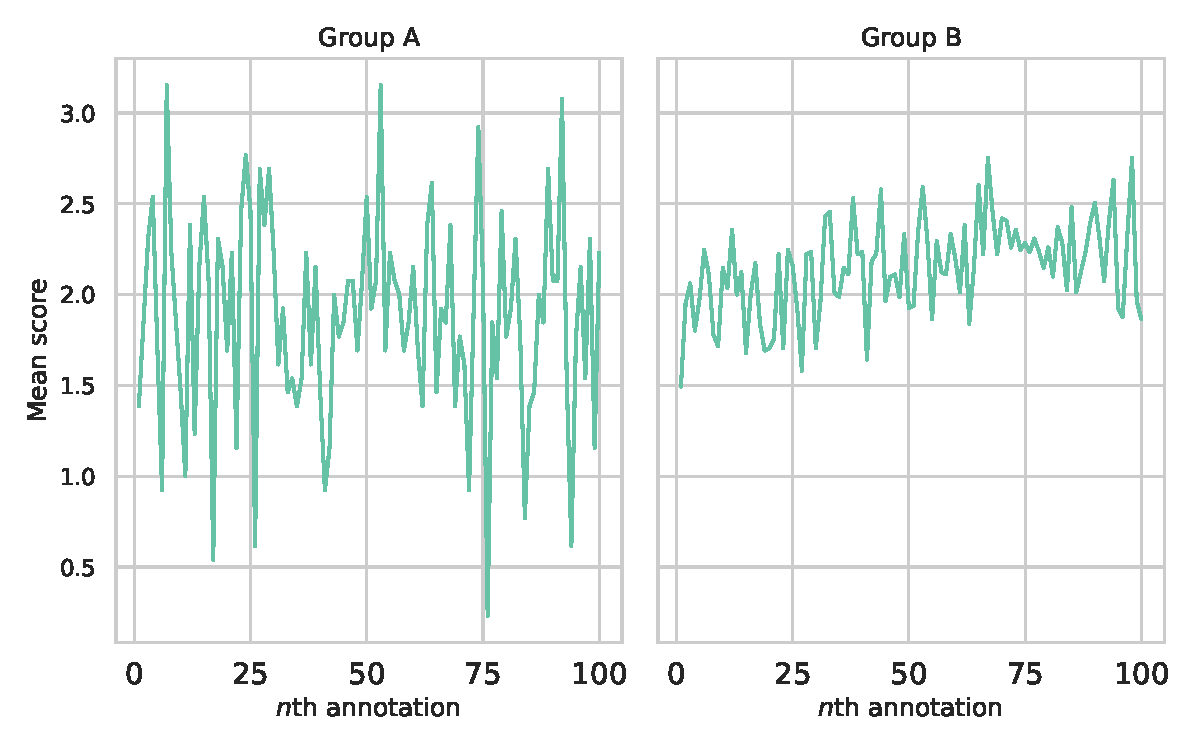
\includegraphics[scale=0.375]{figures/overtime.pdf}
    \caption{Performance over time for the two player groups (\S\ref{sec:players}). Players in Group B, who were given extra instruction and incentives, improved over time while those in Group A did not.}
    \label{fig:skill_over_time}
\end{figure}

\begin{table}[tb]
\small
\centering
\begin{tabular}{SSSSS} \toprule
    {Group} & {$k$} & {$n$} & {Spearman $\rho$}\\ \midrule
    {A} & {50} & {22} & {-0.03} \\
    {A} & {100} & {13} & {-0.06}  \\
    % {A} & {200} & {4} & {-0.03} \\
    \midrule
    {B} & {50} & {88} & {0.29} \\
    {B} & {100} & {81} & {0.42} \\
    % {B} & {200} & {54} & {0.35} \\
    \bottomrule
\end{tabular}
\caption{The Spearman's rank correlation coefficient between the number of annotations performed before the current annotation and the score on the current annotation, for all $n$ players who have performed $k$ or more annotations. Players in Group B, who were given extra instruction and incentives, improved over time while those in Group A did not.}
\label{tab:correlation_over_time}
\end{table}

\begin{figure}[tb]
    \centering
    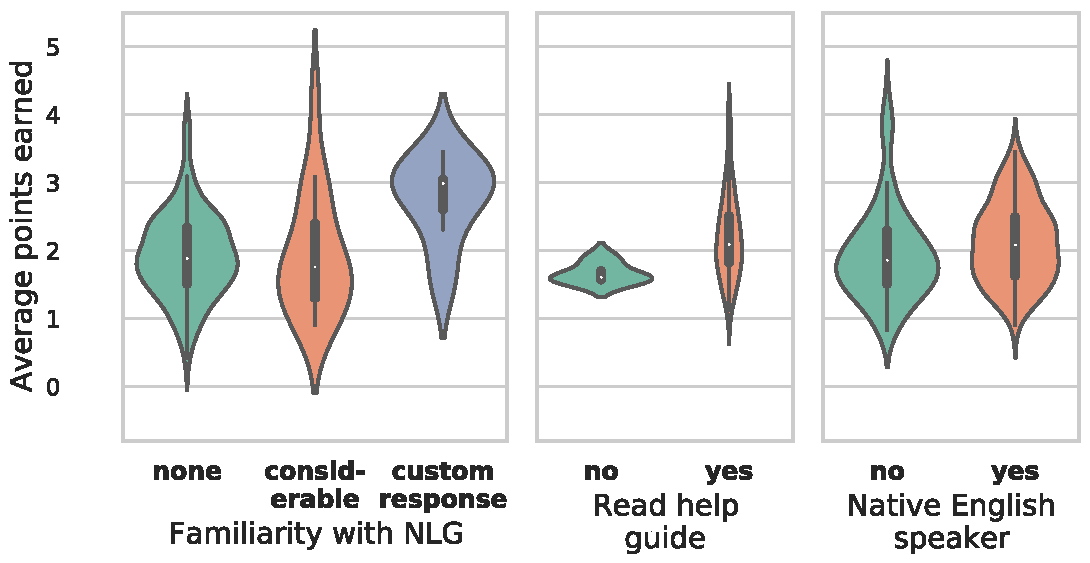
\includegraphics[width=0.5\linewidth]{figures/survey_results_no_fam.pdf}
    \caption{Violin plots showing results of our mandatory exit survey. A violin plot is a box plot that also provides a density estimation. Results shown are filtered to only include players who did at least 20 rounds. We see that reading the help guide, being a native English speaker, and providing a custom response for your familiarity with NLG all contribute to a higher mean score while high domain expertise does not seem have an affect (except in the case of short stories, where variance is lower for domain experts).}
    \label{fig:survey_results}
\end{figure}

\begin{figure}[tb]
    \centering
    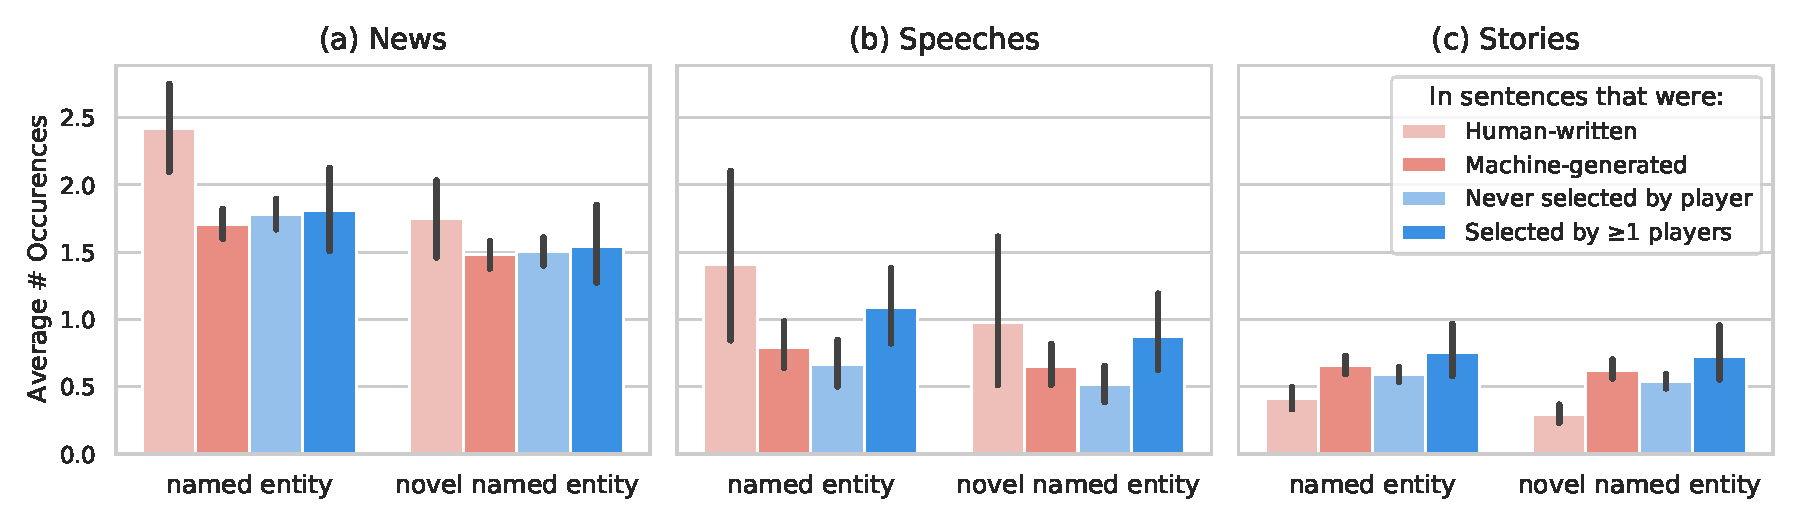
\includegraphics[width=\linewidth]{figures/ner_stats.pdf}
    \caption{We see that human sentences tended to have a different number of named entities than generated sentences.
    Players picked up on the correct trend in Stories, but not in News or Speeches.}
    \label{fig:sentence_stats}
\end{figure}

\begin{figure}[ht]
    \centering
    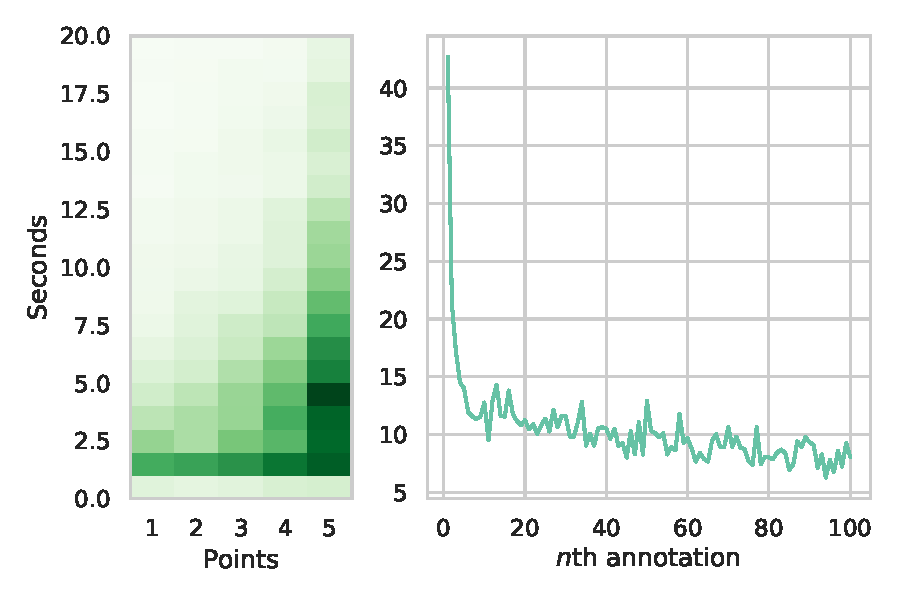
\includegraphics[width=0.7\linewidth]{figures/time_tracking.pdf}
    \caption{\textbf{(left)} Histogram showing the relationship between points earned and the number of seconds an annotation took. Annotators tended to earn more points on annotations they spent longer on.
    \textbf{(right)} Among players who completed at least 100 annotations, average annotation speed decreased with increased experience at the task.
    % We see that high scoring annotations take longer and that players get faster over time.
    % \TODO{nth annotation -> nth game round}
    }
    \label{fig:time_tracking}
\end{figure}


\subsubsection{How much time did game rounds take?}
To understand how much time game rounds took, we logged how many seconds players spent on each sentence decision.
We controlled for instances of players leaving a game open mid-annotation by applying $\min(120, t)$ to all recorded times $t$.
We computed total time per annotation by summing the times for each sentence-level decision.
We found players took longer on annotations where they ended up receiving more points, and players gradually got faster over time (Figure \ref{fig:time_tracking}).
While one might expect longer sentences to take more time to read and make decisions on, we found no correlation between time taken and length of sentence ($\rho$=-0.10), indicating that players take time to think about the task beyond just reading the sentence.

\subsubsection{What sentence-level features could be used to detect generated text?}
It has been well-studied how generated text differs in basic, measurable ways from human-written text, often due to the choice of decoding strategy.
In particular, we measured how sentence length, part-of-speech distribution, and presence of named entities and novel words differed between the generated and human-written sentences in our dataset, and whether players were able to pick up on these differences.
Figure \ref{fig:sentence_stats} shows the results for named entities, where novel named entities are ones which occured in the current sentence but not in any previous sentences.
We found surprisingly different trends across different genres.
On News and Recipes, the generated sentences tended to have fewer named entities than in human-written sentences.
Annotators did not pick up on these trends, though they may have picked up on the fact that for Stories, the generated sentences tended to have slightly more named entities.

In News and Speeches, machine-generated sentences tended to be shorter than human-written ones, a trend players did not pick up on.
However, for Stories, the generated sentences were on average longer than the human ones, and annotators tended to select longer sentences as the boundary.
Additionally in Stories, generated sentences has on average a greater proportion of adjectives and adverbs, but annotators did not pick up on this trend.


\subsubsection{Does familiarity affect detectability?}
All participating players filled out an exit survey after completing their annotations. The questions on this survey are in Table \ref{tab:survey_questions}.
Figure \ref{fig:survey_results} shows some of the results.
First, there was not much difference in performance between participants who reported they had never heard of GPT-2/3 and those who reported having considerable familiarity with them.
Interestingly, participants who answered ``other'' and wrote custom responses did end up being better at the task.
(For example, we released the extra credit assignment a week after a prominent NLG researcher gave a colloquium talk, and a couple responses we received references hearing about them in her talk.)
Second, participants who admitted that they did not read the help guide tended to perform poorly; all the best players did read the guide.
Third, there was not much difference in ability between native and non-native English speakers.
The very strongest players were not native English speakers.
Finally, we did not observe any correlation between self-reported familiarity with a given genre and detection skill on that genre.
% We see that a larger degree of domain familiarity does not have a statistically significant effect on mean score. However, we see that those who did not read the provided help guide did much worse on average and those that gave a custom response to their familiarity with NLG did much better on average. Finally, while native English speakers did do better on average than non-native speakers, the variance for non-natives was much higher resulting in many of our best players being non-native speakers.

\begin{table}
    \centering
    \small
    \begin{tabular}{p{3in}|l}
    \toprule
    Question & Response Type \\
    \midrule
    What did you (or what are you planning to) major/minor in? & Free Text \\\midrule
    Are you a native English speaker? & Yes/No \\\midrule
    How often do you consult a recipe when preparing food? & Daily (5) \\
    & Once to a few times per week (4) \\
    & Once to a few times per month (3) \\
    & Once to a few times per year (2) \\
    & Never (1) \\\midrule
    How often do you read news from credible news publishers (Wall Street Journal, New York Times, etc.)? & Daily (5) \\
    & Once to a few times per week (4) \\
    & Once to a few times per month (3) \\
    & Once to a few times per year (2) \\
    & Never (1) \\\midrule
    How often do you read fiction on the internet (fan fiction, creative writing sub-reddits, ebooks, etc.)? & Daily (5) \\
    & Once to a few times per week (4) \\
    & Once to a few times per month (3) \\
    & Once to a few times per year (2) \\
    & Never (1) \\\midrule
    What is your familiarity with GPT-2 and GPT-3? & I’ve used them before (OpenAI API, HuggingFace, etc.) (4) \\ 
    & I’ve been excitedly following them. (3) \\
    & I've read about them in the news or a blog post. (2) \\
    & I've never heard of them. (1) \\\midrule
    Did you read the RoFT Guide before you tried the game? & Yes/No \\\midrule
    Do you agree for the data being collected on this form along with any annotations you make to be used in an anonymized, aggregated way for research on students' ability to detect machine-generated text? Your answer on this question will not affect your grade. & Yes/No \\
    \bottomrule
    \end{tabular}
    \caption{The text of the exit survey questions given to players after completing their annotations}
    \label{tab:survey_questions}
\end{table}

\subsubsection{What are the most reliable errors to look for when detecting generated text?}
\label{sec:reasons}
Each time a player specified a sentence was machine-generated, they had the option to specify why they made this decision, selecting from a set of pre-defined options (Table \ref{tab:reasons_text}) or else writing down a custom reason.
Table \ref{tab:reasons} shows for each reason, the average number of points earned when that reason was specified.
Like \citet{clark2021all}, we see that conditioning on bad grammar is by far the least reliable way to detect generated text.
In addition, we see that over 30\% of all reasons given for thinking generated text was generated was because the text was ``irrelevant or unrelated to the previous sentences.''
This result stayed consistent across all models and domains.
We note that the three most reliable reasons given (``common\_sense,'' ``irrelevant,'' and ``contradicts\_sentence'') were also the three most common, indicating that improving these attributes will lead to the biggest improvements in generation performance.

Figure \ref{tab:reasons_text} shows the full text of the reasons players could choose between for their boundary decisions, as well as some ``other'' responses we received. 
Figure \ref{fig:reasons_per_model} hows a more detailed breakdown of the percentage of errors made by different models. We see that using $p=1.0$ results in a higher percentage of ``irrelevant'' errors (36\%) than $p=0.0$ (31\%) and $p=0.4$ (28\%) while models decoded using $p=0.0$ in turn have a higher percentage of ``generic'' errors. We also see that smaller models tend to make more ``irrelevant'' errors than larger models (39\% vs. 28\%).
More research is necessary to understand not only the distribution of the types of errors made by certain generative models but also the ways in which that distribution changes given factors such as domain, model size, and decoding strategy.

\begin{table}[tb]
    \centering
    \small
    \begin{tabular}{l|p{30em}}
    \toprule
    Reason & Description \\
    \midrule
    grammar &  is not grammatical \\
    repetition & substantially repeats previous text or itself \\
    irrelevant & is irrelevant or unrelated to the previous sentences \\
    contradicts\_sentence & contradicts the previous sentences \\
    contradicts\_knowledge & contradicts your understanding of the people, events, or concepts involved \\
    common\_sense & contains common-sense or basic logical errors \\
    coreference & mixes up characters' names or other attributes \\
    generic & contains language that is generic or uninteresting \\
    \midrule
    other & $\whitepointerright$Bacon is not sauted \\
     & $\whitepointerright$Mr. vs President Clinton \\
     & $\whitepointerright$navel and sternum seem like very unusual word choices \\
     & $\whitepointerright$It's unlikely that President Nixon will be quoting a one-month old report when he talks about progress made to date   \\
     & $\whitepointerright$lemon, zest of some things dont sound right? 34 cups of splenda and 14 cups of vinegar? \\
     & $\whitepointerright$doesn't rhyme like rest \\
     & $\whitepointerright$Grammar substantially improves from the previous sentences \\
    \bottomrule
    \end{tabular}
    \caption{\textbf{(top)} The possible reasons players could select for why text was machine generated, and \textbf{(bottom)} several examples of custom reasons players wrote.}
    \label{tab:reasons_text}
\end{table}

\begin{figure*}[tb]
    \centering
    \hbox{\hspace{6.0em} 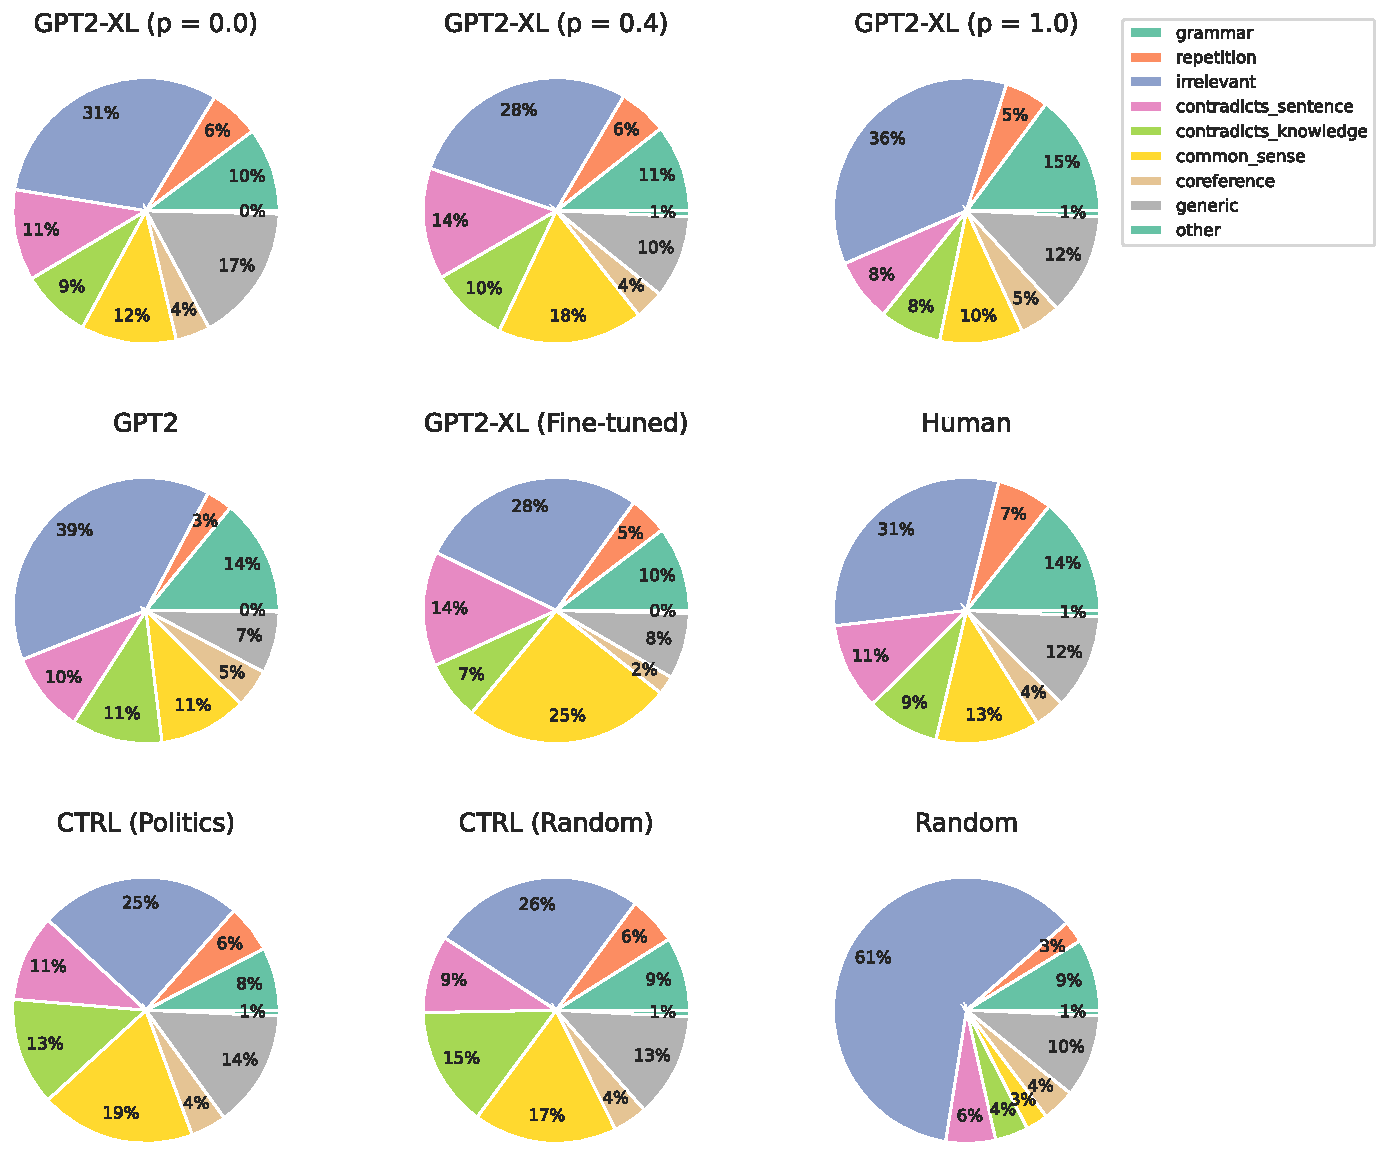
\includegraphics[scale=0.6]{figures/reasons_per_model.pdf}}
    \caption{The reasons provided by players as to why a given example was generated broken up per model that generated the text}
    \label{fig:reasons_per_model}
\end{figure*}

\begin{table}[tb]
\small
\center
\begin{tabular}{lcc} \toprule
    {Reason} & {$n$} & {Mean Score}\\ \midrule
    {common\_sense} & {2,432} & {2.566 $\pm$ 0.086} \\
    {irrelevant} & {4,259} & {2.530 $\pm$ 0.064}  \\
    {contradicts\_sentence} & {1,606} & {2.527 $\pm$ 0.105}  \\ 
    {contradicts\_knowledge} & {1,411} & {2.262 $\pm$ 0.111}   \\
    {coreference} & {542} & {2.249 $\pm$ 0.176} \\
    {repetition} & {728} & {2.128 $\pm$ 0.154} \\
    {other} & {75} & {2.040 $\pm$ 0.483} \\
    {generic} & {1,546} & {1.920 $\pm$ 0.101} \\
    {grammar} & {1,539} & {1.780 $\pm$ 0.105} \\\bottomrule
\end{tabular}
\caption{
The number of times each reason was given for text being machine-generated, and the mean score over those annotations.
We see that when players select reasons like ``grammar'' or ``generic,'' they are much less likely to be correct than when selecting ``common\_sense'' or ``irrelevant.''}
\label{tab:reasons}
\end{table}

\subsection{Discussion}
\label{section:roft_discussion}
In the \ROFT{} user study, we demonstrated the viability of the boundary detection task as a framework for soliciting human evaluation of natural-language generation systems.
We conducted the largest study of generated text detectability to date and, in the process, replicated many previous major results in the field, such as the improved performance of bigger models \citep{kaplan2020scaling} and the difficulty in incentivizing annotators to improve over time \citep{clark2021all}.
We confirmed the result from Section \ref{section:detection} showing that less random decoding strategy settings result in generated text that is harder for humans to detect.
While this trend was true in both domains we tested it in, the impact of deoding strategy was more stark in the Stories domain than the News domain.
In addition, we have provided new insights into the ways in which humans interact with partially-generated text.

Future work could build off out study by testing a larger set of models, genres, and other experimental conditions ((finetuning, topic control, decoding strategy, etc.).
In addition, our study was limited in that we assumed continuations always happened on the sentence boundary, but that is not always necessarily the case.
Future work could look at continuations that do not happen exactly on the boundary between sentences.
We also believe that more investigation is needed into exactly what annotators are thinking when they make their decisions and how we can give annotators the right tools to explain their thought processes.

% Researchers need to help give annotators the language to properly explain how and why they come to select the sentences that they do, whether this be in the form of better error categorization or in free text responses. 

Finally, we expect our released dataset of generations and annotations to be of broad use to those studying detection.
It would be worthwhile to study how well automatic systems perform at the detection task, and whether we can predict when generated text will be especially difficult for human annotators to recognize.

\subsection{Study Limitations}
Work on the detectability of machine-generated text sits at an interesting balancing point.
On one hand, gamifying and publicizing the detection task may help to raise the public's awareness of their susceptibility to machine-generated text, and work such as ours paves the way for future research on techniques for helping the public to improve at detection.
On the other hand, we show that the detection task is a viable method for evaluating generation systems.
For researchers aiming to build better generative language models, decreasing human detection ability might a very reasonable goal to optimize for.
As much as our project seeks to better understand and improve human detection, our results can just as easily be used to make generative models even less detectable than they already are.
Despite this drawback, we nonetheless believe it is important to study detection as a means of assessing the risks that language models pose and protecting against future harm.

One significant limitation in our work is in our choice of participants.
We acknowledge that university students (many of whom have studied computer science) may not be representative of the larger population.
It will be important for future work to take on a broader user study conducted with a more diverse population with the goal of understanding how the unique backgrounds of different annotators contribute to their ability to detect generated text.

Another limitation in our study was in the incentives given to participants to perform well.
Many of the students given extra credit proportional to the amount of points they scored learned they could exploit the point system by always picking one of the later sentences as the boundary.
They found that rapidly guessing Sentence 9 as the boundary on every game round was a more effective strategy for maximizing earned points per time spent than taking the time to carefully read the text in each round.
One alternative system which could reduce this bias would be to show all ten sentences in the passage at once rather than show them one at a time.
The player would get a certain number of tries to guess the index of the boundary sentence and would be scored based on the number of tries this takes.
This would resolve the bug in our current system that some sentence positions have a high point value in expectation.

\section{Conclusion}
In this chapter, I introduce the task of detecting when text is machine-generated.
This task can either be a human evaluation task (asking annotators to identify when text is generated) or an automatic one (building discriminators which can identify it).
In Section \ref{section:detection} I conduct a preliminary study of how humans and finetuned BERT classifiers perform on this task.
I show that decoding strategies which result in generated text that tends to fool humans lead to text that is likely to fool automatic detection systems.
However, the results in this section are limited in that they don't break down detection by text genre, don't investigate passages which are partially human-written and partially generated, and assume the automatic classifiers have access to training data from the same generative model we are aiming to detect samples from.

Section \ref{section:roft} aims to fill in several of these gaps by conducting a lage-scale user study of human detection ability.
In the \ROFT{} user study, I demonstrate the viability of a boundary detection task as a framework for soliciting human evaluation of natural-language generation systems.
I conduct the largest study of generated text detectability to date and, in the process, replicate many previous major results in the field, such as the improved performance of bigger models \citep{kaplan2020scaling} and the difficulty in incentivizing annotators to improve over time \citep{clark2021all}.
We confirmed the result from Section \ref{section:detection} showing that less random decoding strategy settings result in generated text that is harder for humans to detect.
While this trend was true in both domains we tested it in, the impact of decoding strategy was more stark in the Stories domain than the News domain.
In addition, we have provided new insights into the ways in which humans interact with partially-generated text.

Future work could build off our study by testing a larger set of models, genres, and other experimental conditions ((finetuning, topic control, decoding strategy, etc.).
In addition, our study was limited in that we assumed continuations always happened on the sentence boundary, but that is not always necessarily the case.
Future work could look at continuations that do not happen exactly on the boundary between sentences.
We also believe that more investigation is needed into exactly what annotators are thinking when they make their decisions and how we can give annotators the right tools to explain their thought processes.


\section{Summary of Contributions}
My initial research on the detection task was published as ``Automatic Detection of Generated Text is Easiest when Humans are Fooled'' in the 2020 Proceedings of the Association of Computational Linguistics \citep{ippolito2020automatic}.
The work was performed with in conjunction with Daniel Duckworth, with the mentorship of Douglas Eck and Chris Callison-Burch.
I proposed the initial idea of studying detection, and Daniel and I both worked on designing and implementing the experiments and analyzing the results.

The Real or Fake Text annotation platform was introduced as a system demonstration at the 2020 Conference on Empirical Methods in Natural Language Processing \citep{dugan2020roft}.
The RoFT website was implemented by Arun Kirubarajan, Liam Dugan, and myself, with the assistance of Run Shi, and the mentorship or Chris Callison-Burch.
The user study using annotations from RoFt was designed and run, and its results analyzed, by Liam and myself.
